% Created 2010-11-16 Tue 00:46
\documentclass[xcolor=table,bigger]{beamer}
\usepackage[utf8]{inputenc}
\usepackage[T1]{fontenc}
\usepackage{fixltx2e}
\usepackage{graphicx}
\usepackage{longtable}
\usepackage{float}
\usepackage{wrapfig}
\usepackage{soul}
\usepackage{textcomp}
\usepackage{marvosym}
\usepackage{wasysym}
\usepackage{latexsym}
\usepackage{amssymb}
\usepackage{hyperref}
\usepackage{pifont}
\usepackage{IEEEtrantools}
\usepackage{subfig}
\usepackage{tikz}
\usepackage{multirow}
\usetikzlibrary{shapes.geometric, arrows}
\tikzstyle{startstop} = [rectangle, rounded corners, minimum width=3cm, minimum height=1cm,text centered, draw=black, fill=red!30]
\tikzstyle{io} = [trapezium, trapezium left angle=70, trapezium right angle=110, minimum width=3cm, minimum height=1cm, text centered, draw=black, fill=blue!30]
\tikzstyle{process} = [rectangle, minimum width=3cm, minimum height=1cm, text centered, draw=black, fill=orange!30]
\tikzstyle{decision} = [diamond, minimum width=3cm, minimum height=1cm, text centered, draw=black, fill=green!30]
\tikzstyle{arrow} = [thick,->,>=stealth]
\tolerance=1000
\providecommand{\alert}[1]{\textbf{#1}}

\newcommand\vertarrowbox[3][6ex]{%
  \begin{array}[t]{@{}c@{}} #2 \\
  \left\uparrow\vcenter{\hrule height #1}\right.\kern-\nulldelimiterspace\\
  \makebox[0pt]{\scriptsize#3}
  \end{array}%
}
\title{Cosmology with Strong Gravitational Lensing}
\author{Darshan Kumar\\Supervisors: Dr Deepak Jain \& Prof Shobhit Mahajan}
\date{October 2020}

\usepackage{booktabs}
\usepackage[natbib=true, bibstyle=authoryear, citestyle=authoryear-comp]{biblatex}
\usepackage{beamerthemesplit}
\usetheme{progressbar}
\usecolortheme{progressbar}
\institute{\vskip1ex Department of Physics \& Astrophysics\\ \vskip-1ex University of Delhi}
\subtitle{PhD Confirmation Talk-2020}
\definecolor{tableShade}{HTML}{787878}
\definecolor{tableShade2}{HTML}{606060}
\setbeamersize{text margin left=.5cm,text margin right=.5cm}
\progressbaroptions{headline=none, frametitle=ckcompliant}
\newcommand{\myitem}{\item[\vspace{0.5ex}]}
\begin{document}

\maketitle
{}
\begin{frame}{Content}{}
\tableofcontents
\end{frame}

\section{\ding{226} Cosmology Overview}
\begin{frame}
 \frametitle{Cosmology Overview}
 \vspace{3mm}
\ding{74} \textbf{Cosmological Principle:} \\
The Universe is spatially Homogeneous and Isotropic at large scale.
\vspace{2mm}\\
 \ding{74} \textbf{The Friedmann-Lema\^{i}tre-Robertson-Walker Metric:}
$$d s^{2}=-c^{2} d t^{2}+a^{2}(t)\left[\dfrac{d r^{2}}{1-k r^{2}}+r^{2} d \theta^{2}+r^{2} \sin ^{2} \theta d \phi^{2}\right]$$
\begin{flushright}
{\scriptsize where, a(t)=Scale factor, k=-1,0,+1 for open, flat, close universe.}
\end{flushright}
\vspace{2mm}
 \ding{74} \textbf{Einstein’s Equations:}
 $$
 R_{\mu \nu}-\dfrac{1}{2} R g_{\mu \nu}+\Lambda g_{\mu \nu}=\dfrac{8 \pi G}{c^{4}} T_{\mu \nu}
 $$
 \begin{flushright}
 {\scriptsize $R_{\mu\nu}$ =Ricci tensor, $R$=Ricci scaler, $g_{\mu\nu}$ =Metric tensor \& $\Lambda$=Cosmological constant.}
 \end{flushright}
 \vspace{2mm}
  \ding{74} \textbf{ Energy-Momentum Tensor:}
$$
T^{\mu \nu}=(\dfrac{P}{c^2}+\rho) u^{\mu} v^{\nu}+Pg^{\mu \nu}
$$
\begin{flushright}
\begin{scriptsize}
$u^\mu$ and $v^\nu$ are 4-velocity, $P$ and $\rho$ are pressure and density of perfect fluid.
\end{scriptsize}
\end{flushright}
\end{frame}
\newpage
\begin{frame}
 \frametitle{Cosmology Overview}
 \vspace{3mm}
\ding{74} \textbf{Friedmann Equations:} 
\begin{IEEEeqnarray}{rCl}\label{eq:ct1}
$$
3 \dfrac{\dot{a}^{2}+k c^{2}}{a^{2}}-\Lambda c^2=8 \pi G \rho
$$
\end{IEEEeqnarray}
\begin{IEEEeqnarray}{rCl}\label{eq:ct2}
$$2 \dfrac{\ddot{a}}{a}+\dfrac{\dot{a}^{2}+k c^{2}}{a^{2}}-\Lambda c^2=-\dfrac{8 \pi G P}{c^{2}}$$
\end{IEEEeqnarray}
\begin{center}
{\boxed{$$\boldmath{ \underbrace{\dfrac{\ddot{a}}{a}}_{\text{Acceleration}}=\vertarrowbox{-}{\text{slow down expansion}}\underbrace{4\pi G_(\rho+3P)}_{\text{gravity}}\vertarrowbox{+}{\text{speeds up expansion}}\underbrace{\dfrac{\Lambda c^2}{3}}_{\text{cosmological constant}}}$$}}
\end{center}
%\begin{flushright}
%--The Raychaudhuri Equation.
%\end{flushright}
\end{frame}
\newpage
\begin{frame}
 \frametitle{Cosmology Overview}
 \vspace{3mm}
\ding{74} \textbf{Cosmological Redshift:} 
$$z \equiv \dfrac{\lambda_{0}-\lambda_{e}}{\lambda_{e}}~~~~~~~~~~~~~\dfrac{a\left(t_{0}\right)}{a\left(t_{e}\right)} \equiv z+1$$
 \vspace{3mm}
\ding{74} \textbf{Cosmological Density Parameters:} 
$$\Omega_{r0}=\dfrac{8 \pi G \rho_r}{3 H_{0}^{2}};~~~~~\Omega_{m0}=\dfrac{8 \pi G \rho_m}{3 H_{0}^{2}};~~~~~\Omega_{k0}=\dfrac{-kc^2}{H_{0}^{2} a_{0}^{2}};~~~~~\Omega_{\Lambda 0}=\dfrac{\Lambda}{3 H_{0}^{2}}$$
\begin{center}
{\boxed{$$\boldsymbol{\Omega_{r0}+\Omega_{m0}+\Omega_{k0}+\Omega_{\Lambda 0}=1}$$}}
\end{center}
 \vspace{3mm}
\ding{74} \textbf{Hubble Parameter:} 
$$
H(z)\equiv H_0E(z)=H_{0} \sqrt{\Omega_{r0}(1+z)^{4}+\Omega_{m0}(1+z)^{3}+\Omega_{k0}(1+z)^{2}+\Omega_{\Lambda 0}}
$$
\begin{flushright}
\begin{scriptsize}
$H_0=\dfrac{\dot{a}(t)}{a(t_0)}=$Hubble-Lema\^{i}tre Constant

\end{scriptsize}\end{flushright}
\end{frame}

\section{\ding{226} Distances in Cosmology}
\begin{frame}
 \frametitle{Distances in Cosmology}
 \vspace{3mm}
% \ding{74} \textbf{Proper (Physical) Distance:} 
%\begin{figure}[ht!]
%\centering
%\includegraphics[width=60mm]{obs}
%%\caption{An observer at the origin observes a standard candle located at comoving coordinate $(r,~\theta,~\phi)$\\
%%\label{fig:obs}}
%\end{figure} 
% $$
% {\footnotesize d_{p}(t)=\int ds=a(t)\int_{0}^{r} \dfrac{d r}{\left(1-k r^{2}\right)^{1 / 2}}=a(t)\cdot\left\{\begin{array}{ll}{\dfrac{1}{\sqrt{k}} \sin ^{-1}(r \sqrt{k})} & {\text { for } k>0} \\ {r} & {\text { for } k=0} \\ {\dfrac{1}{\sqrt{|k|}} \sinh ^{-1}(r \sqrt{|k|)}} & {\text { for } k<0}\end{array}\right.}
% $$
% \end{frame}
% \begin{frame}
% \frametitle{ Transverse Comoving Distance}
 \vspace{3mm}
\ding{74} \textbf{Comoving Distance: } The distance between two objects remains constant in all epoch if that are moving with Hubble Flow.
$$ d_{c o}=\dfrac{d_{p}}{\left(\dfrac{a(t)}{a\left(t_{0}\right)}\right)}=(1+z) d_{p}$$
where $d_p$ is proper distance.\\
 \ding{74} \textbf{Angular Diameter Distance:} 
$$
 d_{A}\left(z\right)=\dfrac{d_{c o}}{1+z}
 $$
 \ding{74} \textbf{Luminosity Distance:}
 $\bullet$ Property of some class of astronomical object that are same throughout all of spacetime, is absolute luminosity.
 $$d_{L}=d_{c o}^{}(1+z)$$
 \end{frame}

  \begin{frame}
 \frametitle{ Cosmological  Distances}
% \vspace{3mm}
\begin{flushleft}
$ {\scriptsize d_{A(z)}=\dfrac{d_{c o}^{}}{(1+z)}=\dfrac{d_{L}(z)}{(1+z)^{2}}=\left\{\begin{array}{cl}{\dfrac{c}{(1+z) H_{0} \sqrt{\Omega_{k 0}}} \sinh \left(\sqrt{\Omega_{k 0}} \displaystyle\int\limits_{0}^{z} \frac{d z^{\prime}}{E\left(z^{\prime}\right)}\right)} & {\text { for } \Omega_{k 0}>0} \\ {\dfrac{c}{(1+z) H_{0}} \displaystyle\int\limits_{0}^{z} \dfrac{d z^{\prime}}{E\left(z^{\prime}\right)}} & {\text { for } \Omega_{k 0}=0} \\ {\dfrac{c}{(1+z) H_{0} \sqrt{-\Omega_{k 0}}} \sin \left(\sqrt{-\Omega_{k 0}} \displaystyle\int\limits_{0}^{z} \frac{d z^{\prime}}{E\left(z^{\prime}\right)}\right)} & {\text { for } \Omega_{k 0}<0}\end{array}\right.}$
\end{flushleft}
For flat $\Lambda$CDM model: $\Omega_{\mathrm{m0}}=0.3$
\begin{figure}[ht!]
\centering
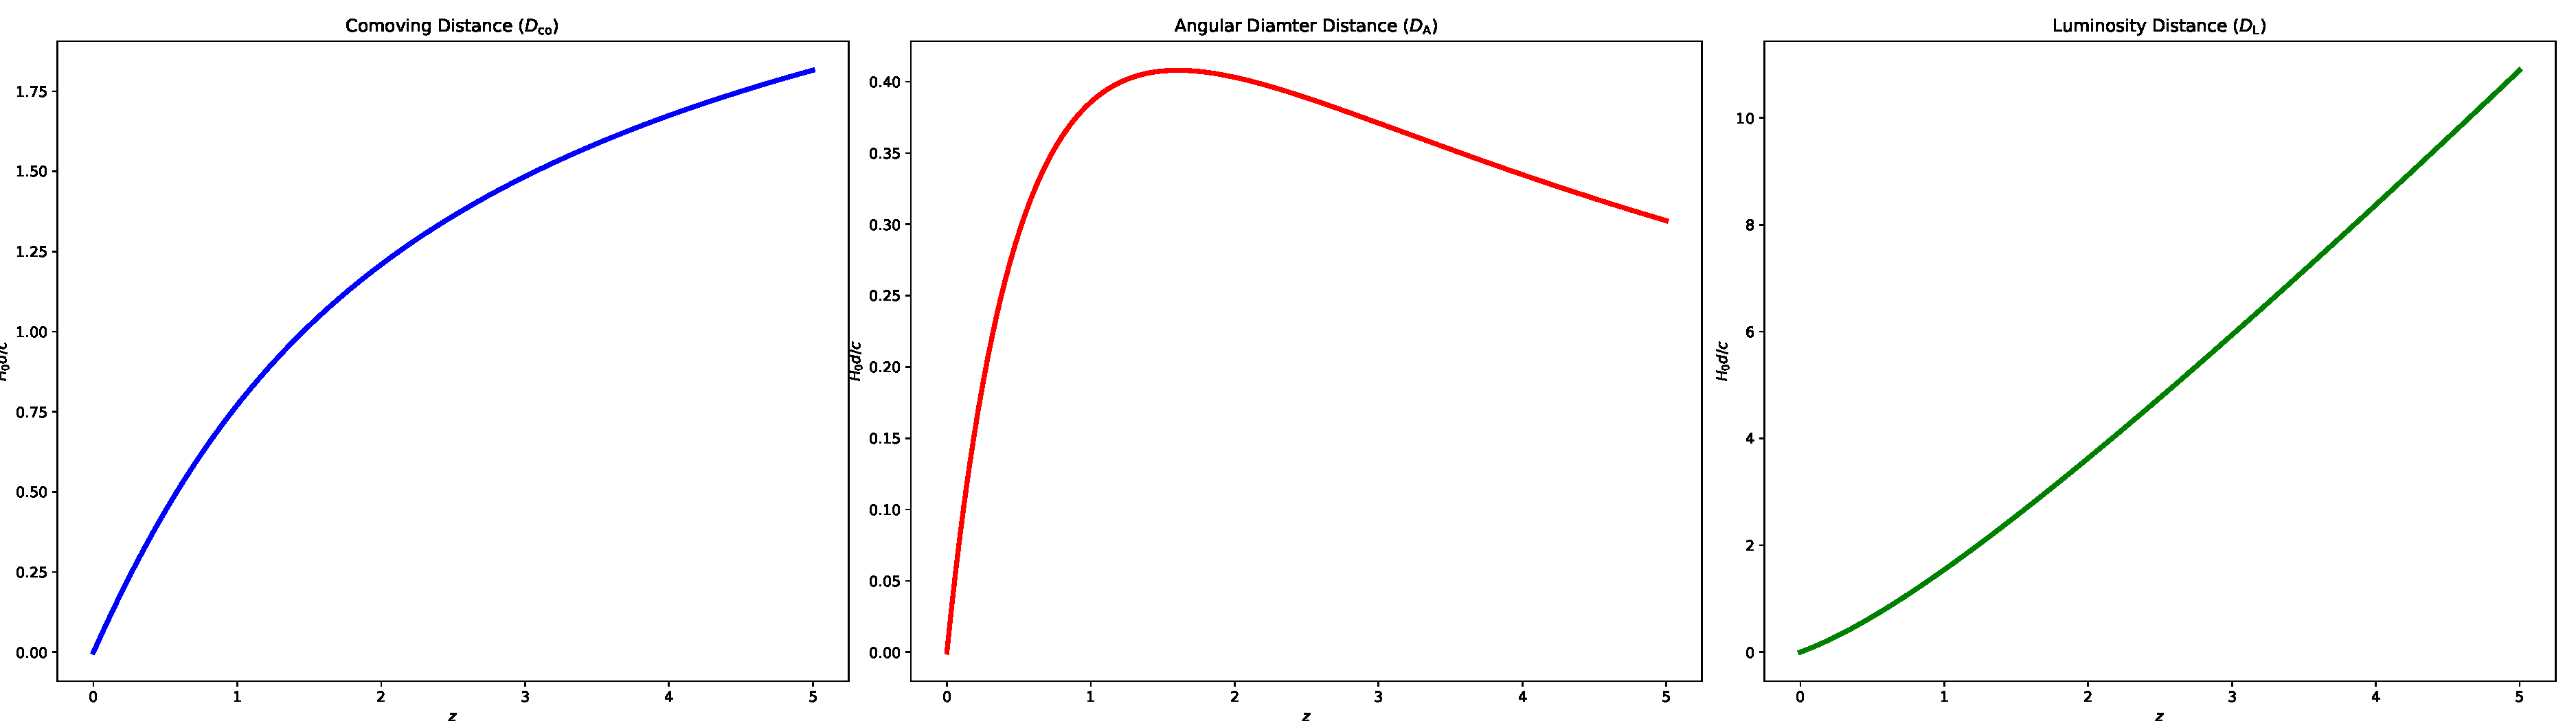
\includegraphics[width=115mm]{d_co_A_L_0_3.pdf}
%\let\thefootnote\relax\footnote{\url{https://www.reddit.com/r/Astronomy}}
\end{figure} 
 \end{frame}
% \section{\ding{226} Distance Sum Rule (DSR) Method}
%\begin{frame}
% \frametitle{Distance Sum Rule}
% \vspace{3mm}
%  \ding{74} For a Non-Euclidean Geometry comoving distance does not follow an additive Relation:
%  $$
%  d_{c o}^{^{z_1z_2}}= d_{c o}^{^{oz_2}} \sqrt{1+\Omega_{k0} \left(\dfrac{H_0}{c}d_{c o}^{^{oz_1}}\right)^{2}}-d_{c o}^{^{oz_1} }\sqrt{1+\Omega_{k0}\left(\dfrac{H_0}{c} d_{c o}^{^{oz_2}}\right)^{2}}
%  $$
%  \hspace{1cm}For $\Omega_{k0}=0$
%  $$
%  d_{c o}^{^{z_1z_2}}=d_{c o}^{^{oz_2}}-d_{c o}^{^{oz_1}}
%  $$
% \ding{74} Even for a flat geometry angular diameter distance doesn't hold additive property:
%$$
%d_{A}^{^{oz_1}}=\dfrac{d_{c o}^{^{oz_1}}}{1+z_{1}} \quad \& \quad d_{A}^{^{oz_2}}=\dfrac{d_{c o}^{^{oz_2}}}{1+z_{2}}
%$$ 
% $$
% d_{A}^{^{z_1z_2}}=a_{z_2}\left(d_{c o}^{^{oz_2}}-d_{c o}^{^{oz_1}}\right) \equiv \dfrac{d_{c o}^{^{z_1z_2}}}{1+z_{2}}\neq d_{A}^{^{oz_2}}-d_{A}^{^{oz_1}}
% $$
% \end{frame}

\section{\ding{226} Strong Gravitational Lensing}
\begin{frame}
 \frametitle{Strong Gravitational Lensing}
\begin{figure}[ht!]
\centering
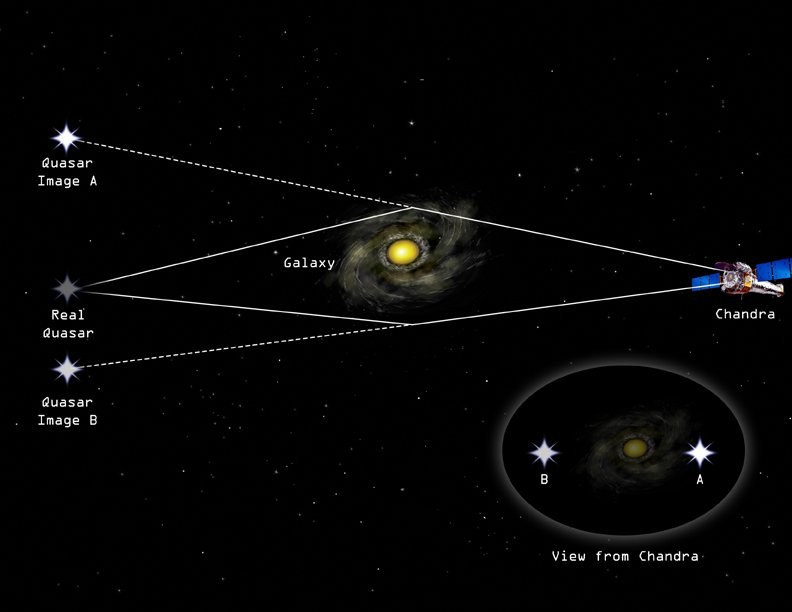
\includegraphics[width=87mm]{cp2}
\let\thefootnote\relax\footnote{\url{https://www.reddit.com/r/Astronomy}}
\end{figure} 
 \end{frame}
 \begin{frame}
 \frametitle{Strong Gravitational Lensing (SGL)}
\ding{74} \textbf{Deflection of light:} Depends only on the gravitational potential of galaxy lens
\vspace{5mm}\\
\ding{74} \textbf{Profile of galaxy lens:}
\vspace{2mm}\\
\begin{itemize}
\item
Singular Isothermal Spherical (SIS)
\vspace{3mm}\\
\item
Power-Law Spherical (PLS)
\vspace{3mm}\\
\item
Extended Power-Law (EPL) Spherical. 
\end{itemize}
 \end{frame}
\begin{frame}
 \frametitle{\textbf{SGL}: Point Mass Lens Profile}

\begin{minipage}{0.45\textwidth}
\ding{74} \textbf{Small Angle Approximation: } All the angles are very small: $\tan{{\theta}}\approx{\theta}$.
\vspace{1mm}\\
\ding{74} \textbf{Weak Field Approximation: }Light passes through a weak field with $\phi\ll\sqrt{c}$.
\vspace{1mm}\\
\ding{74} \textbf{Ray Tracing Equation:} 
$$\beta=\theta-\alpha(\theta)$$
\ding{74} \textbf{Deflection Angle:} 
$$
\hat{\alpha}=\dfrac{4 G M}{c^{2} \xi}
$$
$\Rightarrow$ The deflection angle of Sun :
$$
\hat{\alpha}=\dfrac{4 G M_{\odot}}{c^{2} R_{\odot}}=1.75^{\prime \prime}
$$

\end{minipage}%
\hfill
\begin{minipage}{0.55\textwidth}
\begin{figure}[ht!]
\centering
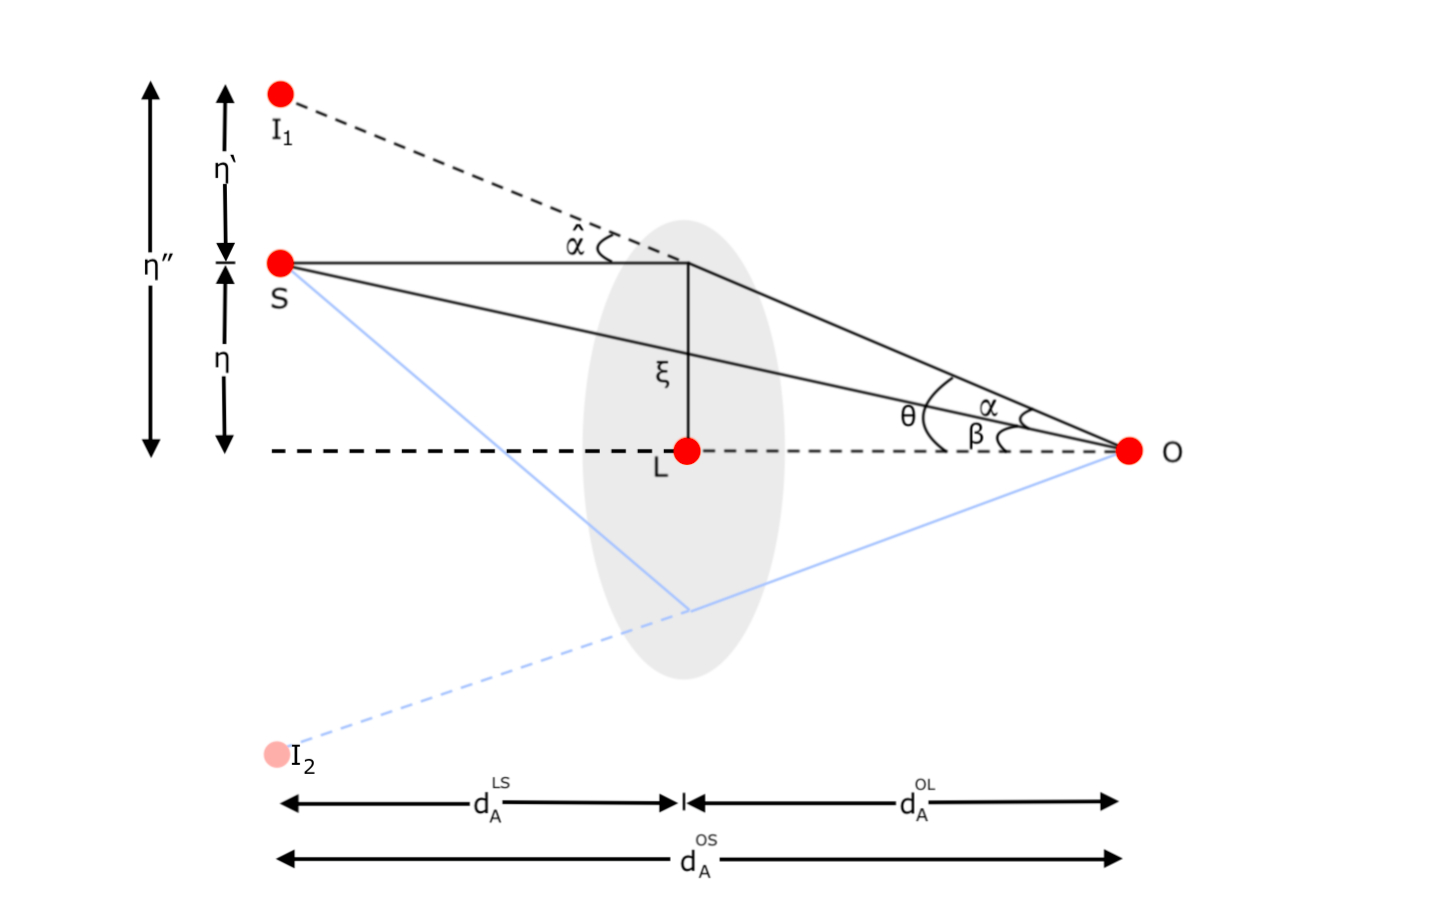
\includegraphics[width=70mm]{sgl1}
%\caption{An observer at the origin observes a standard meter scale, of known proper length $\ell$, at comoving coordinate distance $r$.\\
%\label{fig:angull}}
\end{figure} 
\end{minipage}%
 \end{frame}
\begin{frame}
 \frametitle{\textbf{SGL}: Point Mass Lens Profile:{\large  Einstein Radius}}
\ding{74}
Due to perfect alignment of lens, observer and source, we put $\beta \rightarrow 0$, we obtain the radius of the ring to be
$$
\theta_{E}=\left[\dfrac{4 G M\left(\theta_{E}\right)}{c^{2}} \dfrac{d_{A}^{L S}}{d_{A}^{O L} d_{A}^{o s}}\right]^{1 / 2}
$$
\begin{figure}%
    \centering
    \subfloat[Einstein-Ring]{{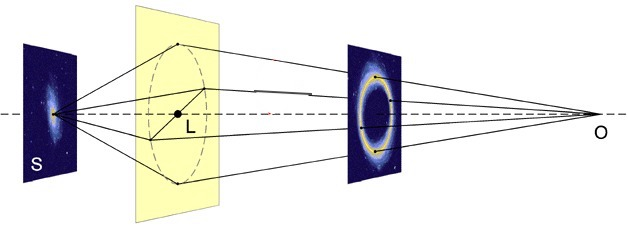
\includegraphics[width=5.5cm]{cp4} }}%
    \qquad
    \subfloat[Arc]{{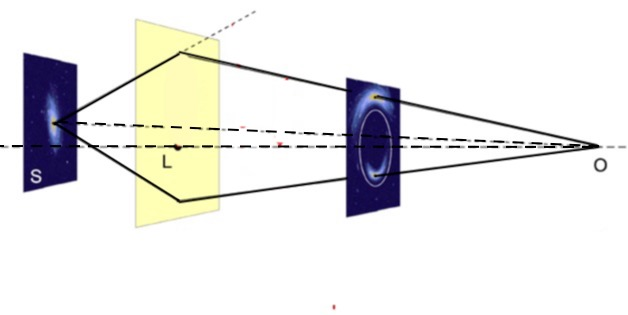
\includegraphics[width=4.0cm]{cp3} }}%
%    \caption{2 Figures side by side}%
%    \label{fig:example}%
\begin{scriptsize}
{(Image: \copyright Google Source)}

\end{scriptsize}
\end{figure}
\ding{74} \textbf{Solution of Lens Equation:}
$$
\beta=\theta-\dfrac{\theta_{E}^{2}}{\theta}~~~~~~~~~~~~~~~~~~~
{\boxed{\theta_{\pm}=\dfrac{1}{2}\left(\beta \pm \sqrt{\beta^{2}+4 \theta_{E}^{2}}\right)}}
$$
 \end{frame}
 \begin{frame}
\begin{center}
%\textbf{Part-A. Distance Ratio}
\vspace{10mm}
\begin{tikzpicture}[node distance=2cm]
\node (start) [startstop] {SGL};
\node (b1) [process, below of=start,left of =start] {Distance Ratio};
\node (b2) [process, right of=b1, xshift=2cm] {Time-Delay Distance};
\node (b3) [process, below of=b1] {$\dfrac{d_{A}^{^{l s}}}{d_{A}^{^{os}}}$};
\node (b4) [process, below of=b2] {$\dfrac{d_{A}^{^{ol}}d_{A}^{^{os}}}{d_{A}^{^{ls}}}$};

\draw [arrow] (start) -- (b1);
\draw [arrow] (start) -- (b2);
\draw [arrow] (b1) -- (b3);
\draw [arrow] (b2) -- (b4);


%\node (pro2b) [process, right of=dec1, xshift=2cm] {Process 2b};

\end{tikzpicture}
\end{center}
 \end{frame}
 \begin{frame}
\begin{center}
\textbf{Part-A. Distance Ratio}
\end{center}
\end{frame}






\begin{frame}
 \frametitle{\textbf{SGL}: {\large Singular Isothermal Spherical (SIS) Lens {\normalsize Profile}}}
 \ding{74} Mass components: {\small Particle of an Ideal gas with velocity dispersion $(\sigma_v)$}.
 \vspace{3mm}\\

\ding{74} Density of mass distribution: $\rho(r)=\dfrac{\sigma_{v}^{2}}{2 \pi G} \dfrac{1}{r^{2}}$
\vspace{3mm}\\

 \begin{minipage}{0.60\textwidth}

%\ding{74} Mass components: {\small Particle of an Ideal gas with velocity dispersion $(\sigma_v)$}.
%\vspace{3mm}\\


\ding{74} Deflection Angle: $\hat{\alpha}=\dfrac{4 \pi \sigma_{v}^{2}}{c^{2}}$
\vspace{4mm}\\

\ding{74} From Einstein Radius: 
$$
{\boxed{\boldsymbol{\dfrac{d_A^{^{ls}}}{d_A^{^{os}}}=\dfrac{c^2\theta_E}{4\pi \sigma_{{v}}^2}}}}
$$
\end{minipage}%
\hfill
\begin{minipage}{0.40\textwidth}
\begin{figure}[ht!]
\centering
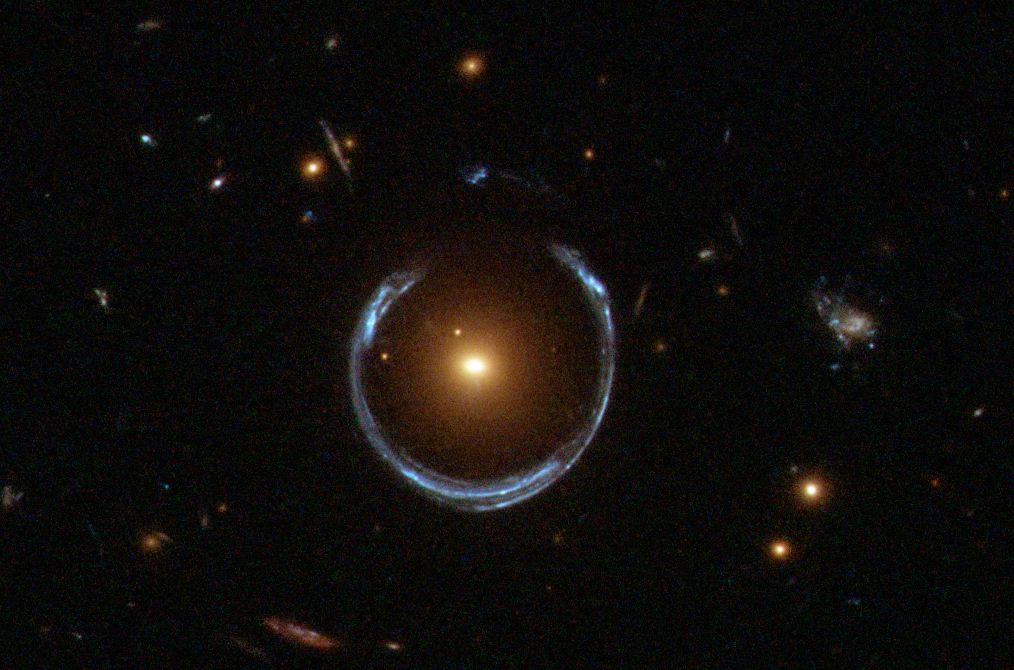
\includegraphics[width=50mm]{Einstein_Ring} \\
%\caption{An observer at the origin observes a standard meter scale, of known proper length $\ell$, at comoving coordinate distance $r$.\\
%\label{fig:angull}}
\begin{scriptsize}
{(Image:\copyright ESA/Hubble/NASA)}

\end{scriptsize}\end{figure} 
%\let\thefootnote\relax\footnote{\url{https://www.reddit.com/r/Astronomy}}

\end{minipage}%
\end{frame}
\begin{frame}
 \frametitle{\textbf{SGL}: { {\large Power-Law Spherical (PLS) Lens Profile}}}
\ding{74} Mass Density:  $~~~~~~~~~~~~~\rho(r)=\rho_{0}\left(\dfrac{r}{r_{0}}\right)^{-\gamma}$ 
\vspace{3mm}\\
Using the \textbf{Spherical Symmetric Jeans Equations:} 
$$
{\boxed{\boldsymbol{d_{AR} \equiv \dfrac{d_{A}^{^{l s}}}{d_{A}^{^{os}}}=\dfrac{c^{2} \theta_{E}}{4 \pi \sigma_{\mathrm{ap}}^{2}}\left(\dfrac{\theta_{a p}}{\theta_{E}}\right)^{2-\gamma} f^{-1}(\gamma)}}}
$$
\vspace{3mm}\\
 where,
 $f(\gamma)=-\frac{1}{\sqrt{\pi}} \frac{(5-2 \gamma)(1-\gamma)}{3-\gamma} \frac{\Gamma(\gamma-1)}{\Gamma(\gamma-3 / 2)}\left[\frac{\Gamma(\gamma / 2-1 / 2)}{\Gamma(\gamma / 2)}\right]^{2}$\\
\end{frame}
\begin{frame}
 \frametitle{\textbf{SGL}: {\normalsize Extended Power-Law (EPL) Spherical Lens Profile}}
\ding{74} Total Mass Density:  $~~~~~~~~~~~~~\rho(r)=\rho_{0}\left(\dfrac{r}{r_{0}}\right)^{-\gamma}$ 
\vspace{2mm}\\
\ding{74} Luminous Mass Density: $~~~~~\nu(r)=\nu_{0}\left(\dfrac{r}{r_{0}}\right)^{-\delta}$
\vspace{2mm}\\
\ding{74} Anisotropic Parameter: $~~~~~~~~\beta(r)=1-\dfrac{\sigma_{\theta}^{2}}{ \sigma_{r}^{2}}$
\vspace{3mm}\\
Using the \textbf{Spherical Symmetric Jeans Equations:} 
$$
{\boxed{\boldsymbol{d_{\mathrm{AR}} \equiv \dfrac{d_{A}^{^{ls}}}{d_{A}^{^{os}}}=\dfrac{c^{2} \theta_{E}}{4 \pi \sigma_{0}^{2}}\left(\dfrac{\theta_{\mathrm{ap}}}{\theta_{\mathrm{E}}}\right)^{2-\gamma} \times f(\gamma, \delta, \beta)}}}
$$
 where,
 $f(\gamma, \delta, \beta)=\frac{(2 \sqrt{\pi})(3-\delta)}{(\xi-2 \beta)(3-\xi)} \times\left[\frac{\Gamma[(\xi-1) / 2]}{\Gamma(\xi / 2)}-\beta \frac{\Gamma[(\xi+1) / 2]}{\Gamma[(\xi+2) / 2]}\right] \frac{\Gamma(\gamma / 2) \Gamma(\delta / 2)}{\Gamma(\gamma-1) / 2 \Gamma[(\delta-1) / 2]}$\\
 \begin{flushright}
 $\xi=\gamma+\delta-2$
 \end{flushright}
\end{frame}
\begin{frame}
 \frametitle{{SGL}: {\normalsize \textbf{EPL} to \textbf{ Power-Law Spherical (PLS) }and \textbf{SIS} Lens Profile}}
\ding{74} \textbf{ PLS Lens Model}
\vspace{2mm}\\
Total Mass Density: $\rho(r)=\rho_{0}\left(\dfrac{r}{r_{0}}\right)^{-\gamma};~~~~~~ \gamma=\delta$
$$
{\boxed{\boldsymbol{d_{\mathrm{AR}}\equiv\dfrac{d_{A}^{^{l s}}}{d_{A}^{^{o s}}}=\dfrac{c^{2} \theta_{E}}{4 \pi \sigma_{ap}^{2}}\left(\dfrac{\theta_{a p}}{\theta_{E}}\right)^{2-\gamma} f^{-1}(\gamma)}}}
$$
\begin{flushright}
where, $f(\gamma)=-\frac{1}{\sqrt{\pi}} \frac{(5-2 \gamma)(1-\gamma)}{3-\gamma} \frac{\Gamma(\gamma-1)}{\Gamma(\gamma-3 / 2)}\left[\frac{\Gamma(\gamma / 2-1 / 2)}{\Gamma(\gamma / 2)}\right]^{2}$
\end{flushright}
%\vspace{3mm}\\
\ding{74} \textbf{ SIS Lens Model}
\vspace{2mm}\\
$\gamma=\delta=2~~~~\text{and}~~~~\beta=0$
$$
{\boxed{\boldsymbol{d_{\mathrm{AR}}\equiv\dfrac{d_A^{^{ls}}}{d_A^{^{os}}}=\dfrac{c^2\theta_E}{4\pi \sigma_{\mathrm{SIS}}^2}}}}
$$
\begin{flushright}
  where, $\sigma_{\mathrm{SIS}}=f_e\sigma_0$

 \end{flushright} \end{frame}
 \begin{frame}
 \frametitle{DSR Method in Distance Ratio}
 \vspace{3mm}
  \ding{74} For a Non-Euclidean geometry, comoving distances do not follow an additive Relation:
  $$
  d_{c o}^{^{\mathrm{ls}}}= d_\mathrm{c o}^{^\mathrm{os}} \sqrt{1+\Omega_{k0} \left(\dfrac{H_0}{c}d_\mathrm{c o}^\mathrm{^{ol}}\right)^{2}}-d_\mathrm{c o}^{^\mathrm{ol} }\sqrt{1+\Omega_{k0}\left(\dfrac{H_0}{c} d_\mathrm{c o}^{^\mathrm{os}}\right)^{2}}
  $$
%  \hspace{1cm}For $\boldsymbol{\Omega_{k0}=0}$
%  $$
%  d_\mathrm{c o}^{^{ls}}=d_\mathrm{c o}^{^\mathrm{os}}-d_\mathrm{c o}^{^\mathrm{ol}}
%  $$
  \ding{74}  Cosmic Distance Duality Relation:  $d_\mathrm{A}=\dfrac{d_\mathrm{c o}}{1+z}=\dfrac{d_\mathrm{L}}{(1+z)^{2}}$
  \vspace{3mm}\\
 \ding{74}DSR in term of Distance ratio:
 \vspace{1mm}\\
\begin{footnotesize}
$$
{\boxed{\boldsymbol{\dfrac{d_{c o}^{^{\mathrm{ls}}}}{d_{c o}^{^{\mathrm{os}}}}\equiv\dfrac{d_{A}^{^{\mathrm{ls}}}}{d_{A}^{^{\mathrm{os}}}}= \sqrt{1+\Omega_{k0} \left(\dfrac{H_0d_\mathrm{L}^\mathrm{^{ol}}}{c(1+z_l)}\right)^{2}}-\dfrac{d_\mathrm{L}^{^\mathrm{ol} }(1+z_s)}{ d_\mathrm{L}^{^\mathrm{os}}(1+z_l)}\sqrt{1+\Omega_{k0}\left(\dfrac{H_0d_\mathrm{L}^{^\mathrm{os}}}{c(1+z_s)} \right)^{2}}}}}
 $$
\end{footnotesize}
 \end{frame}
 \section{\ding{226} Observational Dataset}
\begin{frame}
 \frametitle{Observational Dataset-I}

 \ding{74} \textbf{For Luminosity distance in DSR method:} Pantheon (SNIa)+GRBs datasets: 1048+147 data points: $z\in[0.01,3.6]$
 \begin{figure}[ht!]
\centering
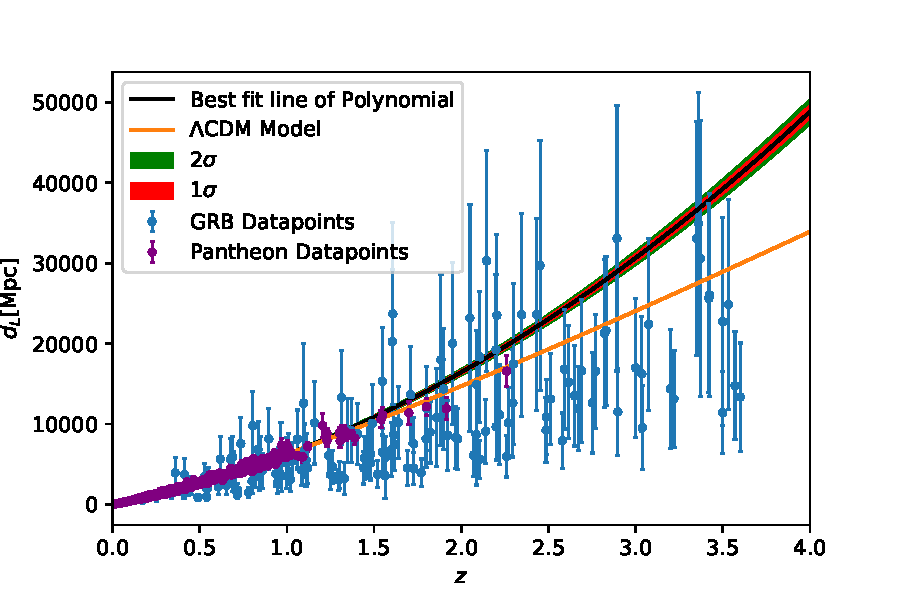
\includegraphics[width=100mm]{Pantheon_GRB_Polynomial_2nd_1048_147_dl}
%\caption{An observer at the origin observes a standard meter scale, of known proper length $\ell$, at comoving coordinate distance $r$.\\
%\label{fig:angull}}
\end{figure} 
 \end{frame}
\begin{frame}
 \frametitle{Observational Dataset-II}
\ding{74} \textbf{For distance ratio in SGL systems:} 161 data points: \hspace*{3 cm}$z_l\in[0.0625,1.004]$ and \hspace*{0 cm}$z_s\in[0.197, 3.595]$
 \vspace{2mm}\\
\ding{74} \textbf{Statistical tools:}
 \begin{figure}[ht!]
\centering
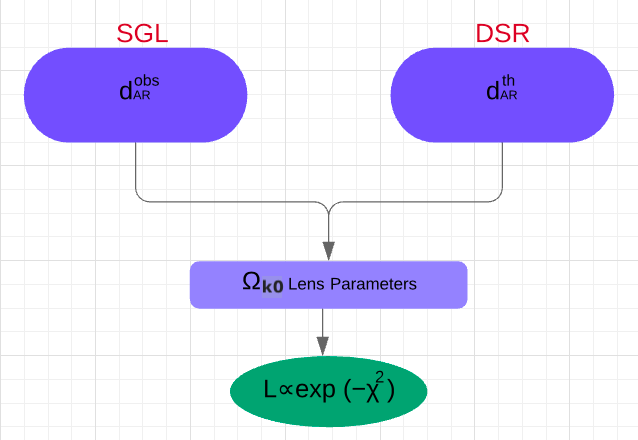
\includegraphics[width=88mm]{flowchart_eicp}
%\caption{An observer at the origin observes a standard meter scale, of known proper length $\ell$, at comoving coordinate distance $r$.\\
%\label{fig:angull}}
\end{figure} 
 \end{frame}
\section{\ding{226} Results and Conclusions}
\begin{frame}
 \frametitle{Results: \textbf{SIS} Lens Model}
 $
{\boxed{\boldsymbol{\dfrac{d_A^{^{ls}}}{d_A^{^{os}}}=\dfrac{c^2\theta_E}{4\pi f_e\sigma_{{0}}^2}}}}
$ \hspace*{2cm}$\begin{array}
 {|l|l|l|}\hline 
 \text { Parameter } & {\text { Best value }[68 \% \mathrm{CL}]} \\ \hline 
 \Omega_{k0} & {0.680^{+0.144}_{-0.136}} \\ \hline f_{e} & {1.034^{+0.006}_{-0.006}} \\ \hline
 \end{array}$
 \begin{figure}[ht!]
\centering
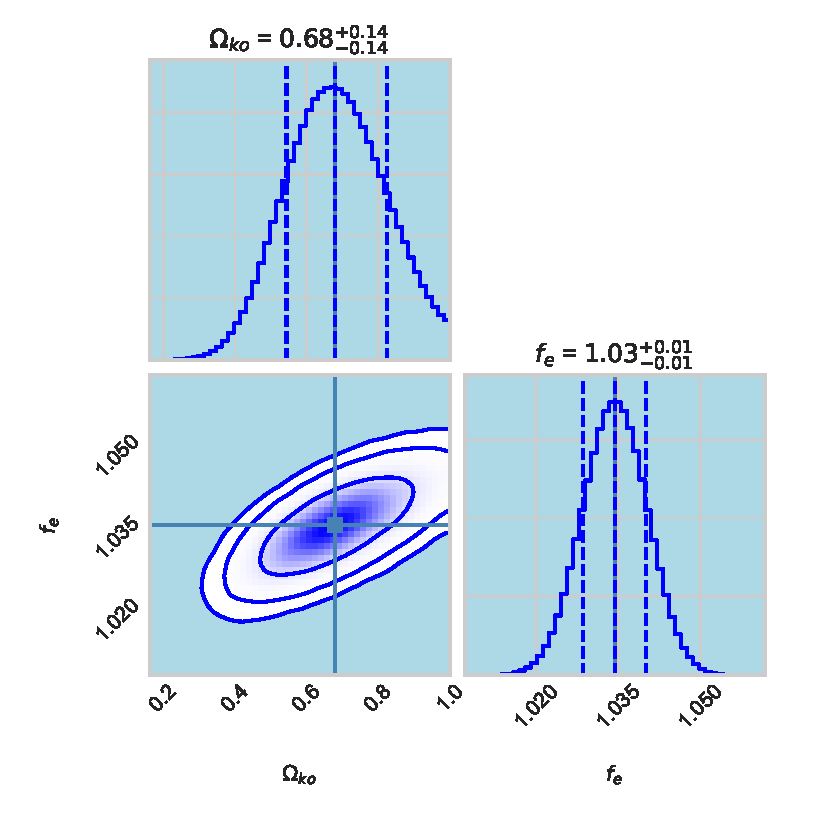
\includegraphics[width=60 mm]{distance_Ratio_161_ok_1_fe_corner_without_H0_dec}
%\caption{An observer at the origin observes a standard meter scale, of known proper length $\ell$, at comoving coordinate distance $r$.\\
%\label{fig:angull}}
\end{figure} 
 \end{frame}
 \begin{frame}
 \frametitle{Results: \textbf{PLS} Lens Model}
\begin{scriptsize}
  $
{\boxed{\boldsymbol{d_{\mathrm{AR}}\equiv\dfrac{d_{A}^{^{l s}}}{d_{A}^{^{o s}}}=\dfrac{c^{2} \theta_{E}}{4 \pi \sigma_{ap}^{2}}\left(\dfrac{\theta_{a p}}{\theta_{E}}\right)^{2-\gamma} f^{-1}(\gamma)}}}
$
 \end{scriptsize}
 {\footnotesize $\begin{array}{|c|c|}\hline \text { Parameter } & {\text { Best value }[68 \% \mathrm{CL}]} \\ \hline \Omega_{k 0} & {-0.052^{+0.054}_{-0.018}} \\ \hline \gamma_{0} & {2.107_{-0.020}^{+0.018}} \\ \hline \gamma_{1} & {-0.371_{-0.062}^{+0.088}} \\ \hline\end{array}$}
  \begin{figure}[ht!]
\centering
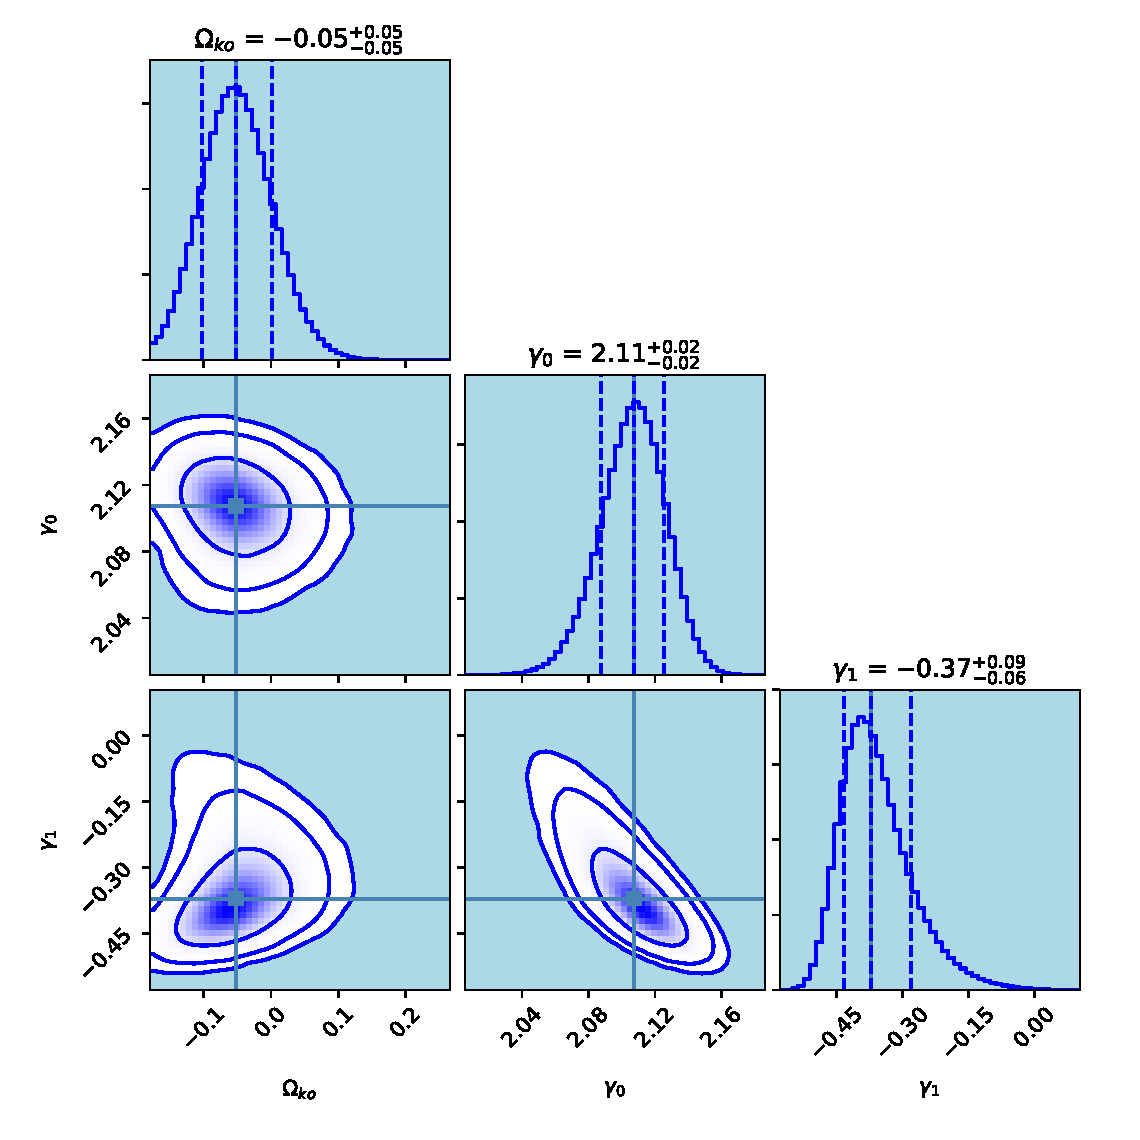
\includegraphics[width=58 mm]{distance_Ratio_161_ok_1_ga0_ga1_corner_without_H0_dec}
%\caption{An observer at the origin observes a standard meter scale, of known proper length $\ell$, at comoving coordinate distance $r$.\\
%\label{fig:angull}}
\end{figure} 
\end{frame}
\begin{frame}
 \frametitle{Results: \textbf{ P1: EPL} Lens Model}
\begin{scriptsize}
$
{\boxed{\boldsymbol{d_{\mathrm{AR}} \equiv \dfrac{d_{A}^{^{ls}}}{d_{A}^{^{os}}}=\dfrac{c^{2} \theta_{E}}{4 \pi \sigma_{0}^{2}}\left(\dfrac{\theta_{\mathrm{ap}}}{\theta_{\mathrm{E}}}\right)^{2-\gamma} \times f(\gamma, \delta, \beta)}}}
$
\end{scriptsize} {\scriptsize $\begin{array}{|c|c|}\hline \text { Parameter } & {\text { Best value }[68 \% \text { C.L. }]} \\ \hline \Omega_{k 0} & {-0.007^{+0.117}_{-0.097}} \\ \hline \gamma_{0} & {2.139^{+0.022}_{-0.021}} \\ \hline \delta & {2.265^{+0.146}_{-0.194}} \\ \hline\end{array}$}
\begin{figure}[ht!]
$\beta=\mathcal{N}\left(0.18,0.13\right)$
\centering
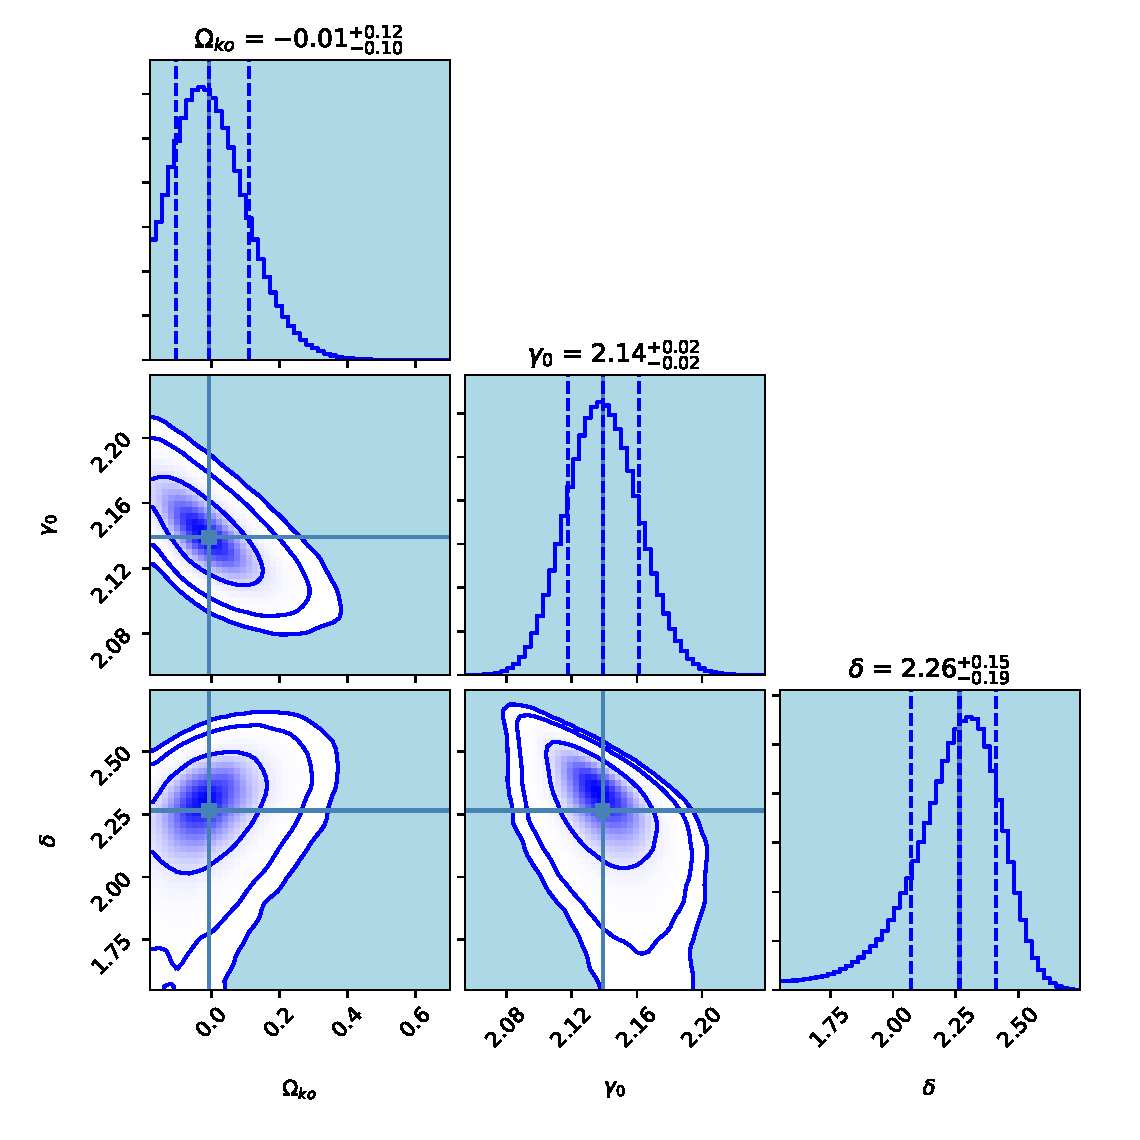
\includegraphics[width=58 mm]{distance_Ratio_161_ok_1_ga_delt_corner_P1_without_beta_h0_dec}
%\caption{An observer at the origin observes a standard meter scale, of known proper length $\ell$, at comoving coordinate distance $r$.\\
%\label{fig:angull}}
\end{figure} 
\end{frame}
\begin{frame}
 \frametitle{Results: \textbf{ P2: EPL} Lens Model}
\begin{large}

$
{\boxed{\boldsymbol{\gamma(z_l)=\gamma_0+\gamma_1 z_l}}}
$
\end{large}\hspace*{1cm}$\begin{array}{|l|r|}\hline \text { Parameter } & {\text { Best value }[68 \% \mathrm{C.L.}]} \\ \hline \Omega_{k 0} & {-0.004^{+0.184}_{-0.118}} \\ \hline \gamma_{0} & {2.154^{+0.043}_{-0.034}} \\ \hline \gamma_{1} & {-0.037^{+0.075}_{-0.094}} \\ \hline \delta & {2.108^{+0.221}_{-0.325}} \\ \hline\end{array}$
\begin{figure}[ht!]
\centering
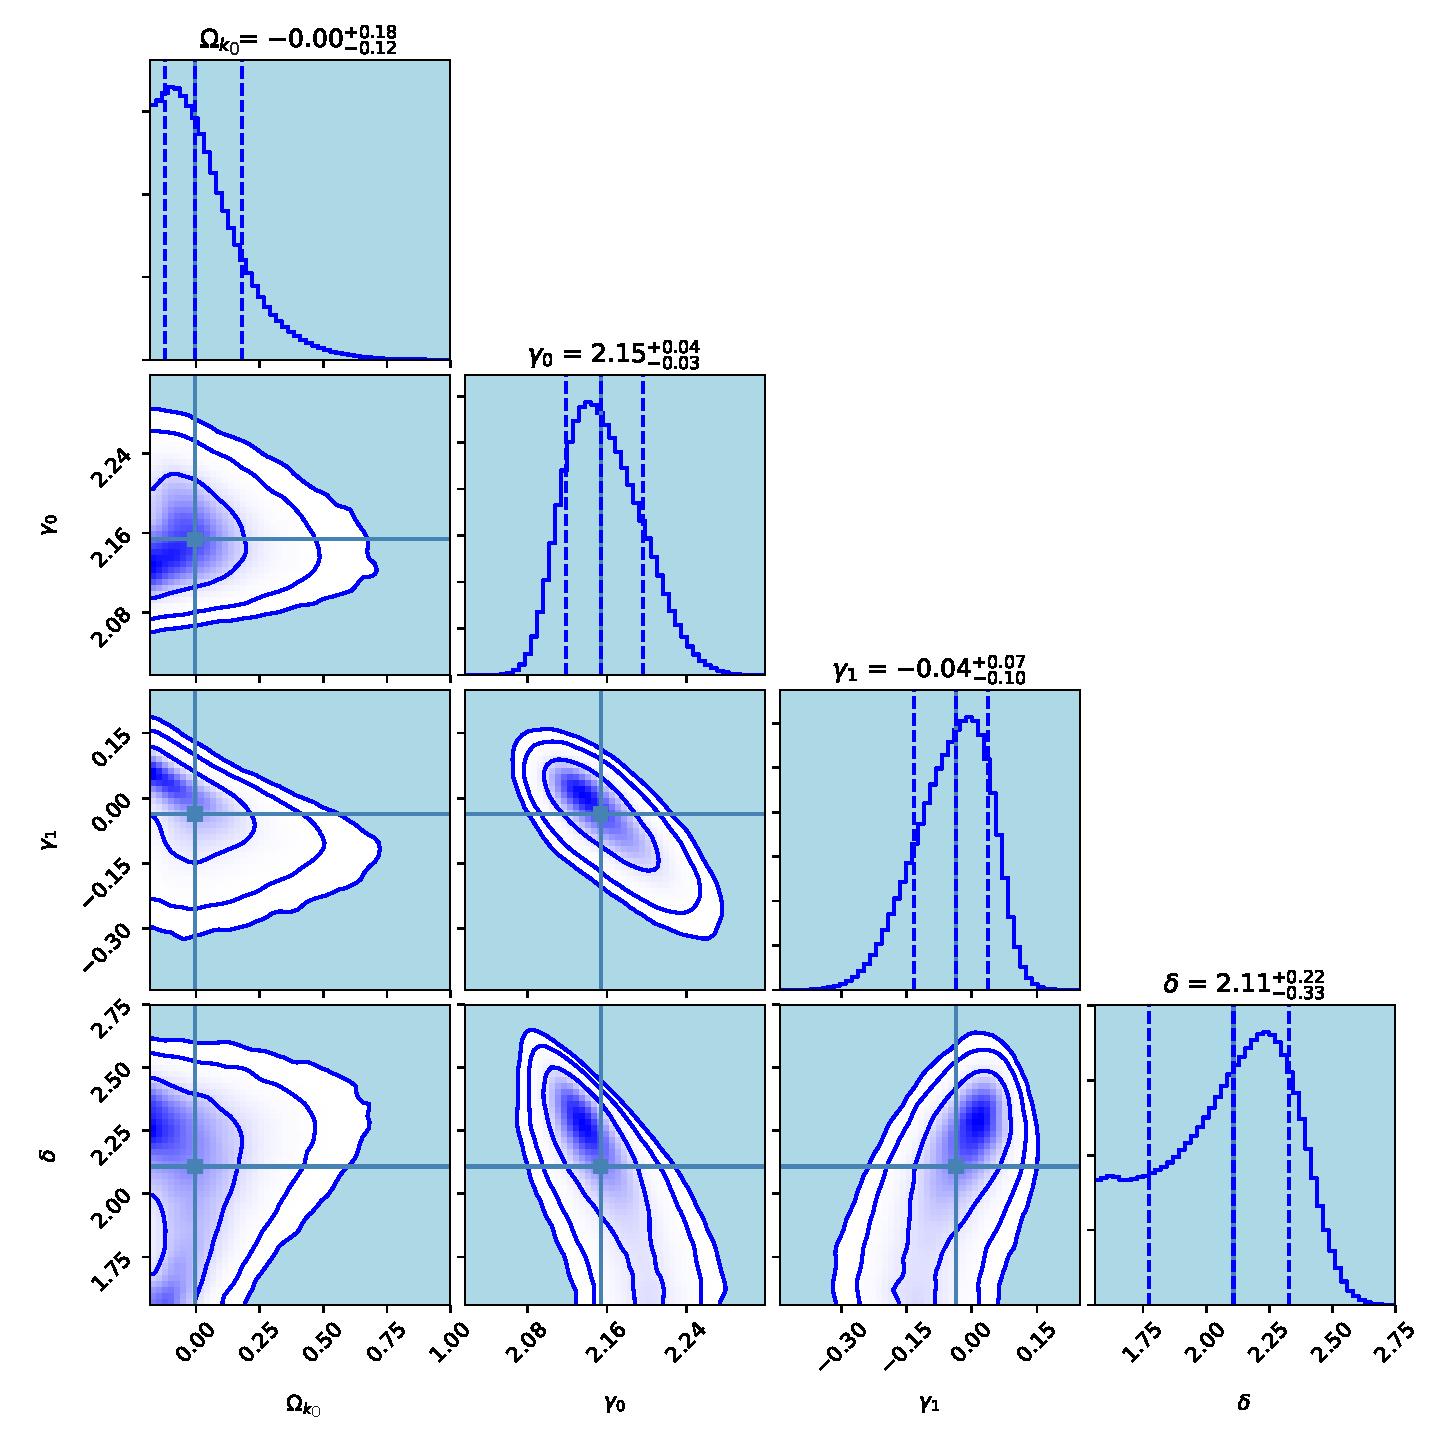
\includegraphics[width=52 mm]{distance_Ratio_161_ok_1_ga0_ga1_delt_P2_corner_without_beta_h0_decc}
%\caption{An observer at the origin observes a standard meter scale, of known proper length $\ell$, at comoving coordinate distance $r$.\\
%\label{fig:angull}}
\end{figure} 
\end{frame}
\begin{frame}
 \frametitle{Results: \textbf{ P3: EPL} Lens Model}
\begin{scriptsize}
$
{\boxed{\boldsymbol{\gamma(z_l)=\gamma_{0}+\gamma_{1} \dfrac{z_{l}}{1+z_{l}}}}}
$
\end{scriptsize}\hspace*{1cm} $\begin{array}{|l|r|}\hline \text { Parameter } & {\text { Best value }[68 \% \mathrm{C.L.}]} \\ \hline \Omega_{k 0} & {-0.032^{+0.168}_{-0.104}} \\ \hline \gamma_{0} & {2.163^{+0.066}_{-0.052}} \\ \hline \gamma_{1} & {-0.083^{+0.184}_{-0.243}} \\ \hline \delta & {2.064^{+0.265}_{-0.353}} \\ \hline\end{array}$



\begin{figure}[ht!]
\centering
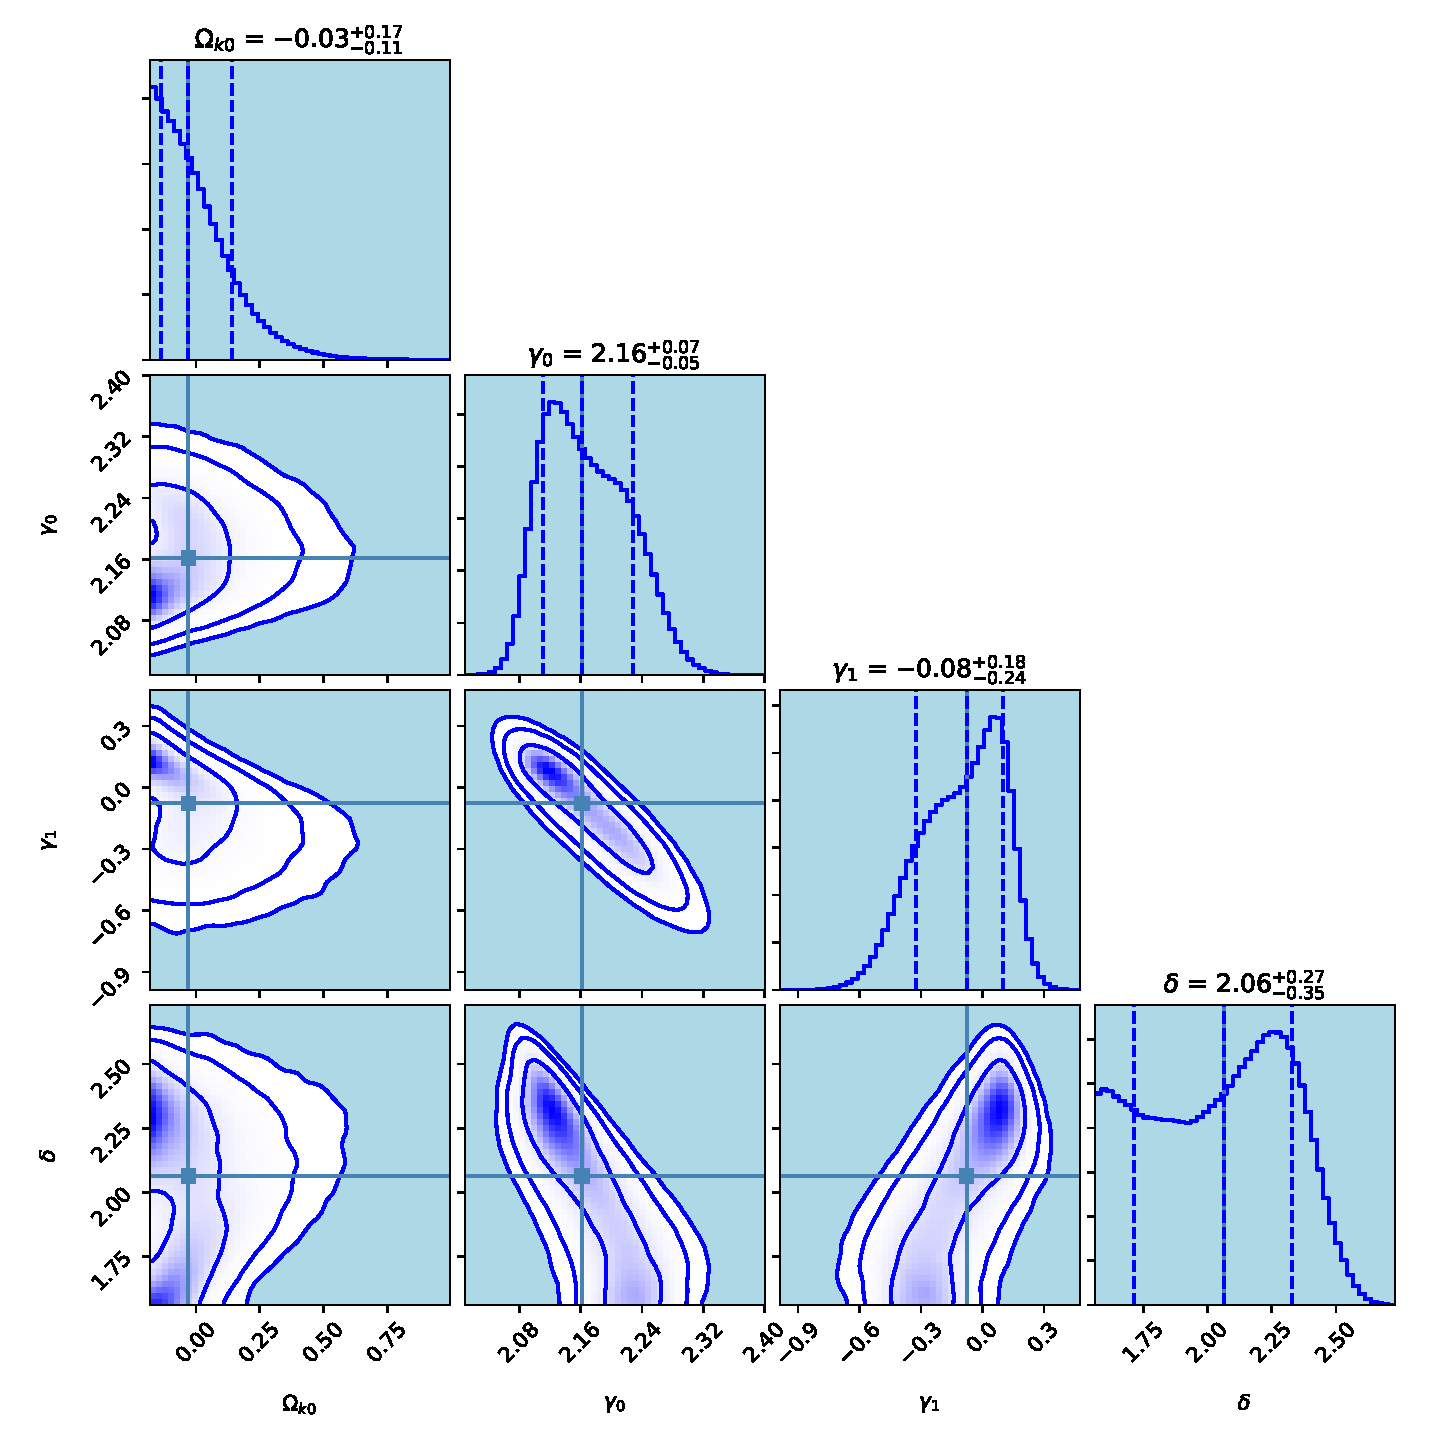
\includegraphics[width=52 mm]{distance_Ratio_161_ok_1_ga0_ga1_delt_P3_corner_without_beta_h0_dec}
%\caption{An observer at the origin observes a standard meter scale, of known proper length $\ell$, at comoving coordinate distance $r$.\\
%\label{fig:angull}}
\end{figure} 
\end{frame}
\begin{frame}
 \frametitle{Conclusions}
 \begin{itemize}
 \item
 \textbf{\small {\color{red}{SIS model}}: We obtain a weak constraint on the cosmic curvature parameter $(\Omega_{k0})$ because of a strong correlation between $(\Omega_{k0})$ and $f_e$.}
 \item
\texttt{\small {\color{red}{PLS model}}: Result indicates that the mass density profile of massive galaxies has become steeper over cosmic time.}
\vspace{1mm}\\
\item
\textbf{\small {\color{red}{EPL model}}: In the P1 parametrisation, for an arbitrary constant $\gamma$ we obtain different values of $\gamma$ and $\delta$, which indicate that the mass density distributions of dark matter and luminous matter are different in early-type galaxies.}
\vspace{1mm}\\
\item
\texttt{\small The results obtained in P2 and P3 suggest that with cosmic time, the total density profile of early-type galaxies can evolve. }
\vspace{1mm}\\
\item
%\fontfamily{verdana}
\textbf{\small The inclusion of a redshift dependent $\gamma$ in the analysis indicates a spatially close universe but can also accommodate the flat universe within 68\% confidence region.}

 \end{itemize}
 
 \end{frame}
\begin{frame}
\vspace{5mm}
\begin{center}
\textbf{Part-B. Time Delay Distance}
\end{center}
\end{frame} 
 \begin{frame}
  \frametitle{Time Delay in SGL}
  \vspace{4mm}
 \ding{74} \textbf{The Geometric Time Delay:} Light path have different path length from source to observer.
 \vspace{6mm}\\
  \ding{74} \textbf{The Gravitational Time Delay:} Light path passes through different gravitational potential of lens.
\vspace{6mm}
\begin{center}
\begin{tikzpicture}[node distance=2cm]
\node (start) [startstop] {Total Time Delay= Geometric Time Delay+ Gravitational Time Delay};
\end{tikzpicture}
\end{center}
\end{frame}
\begin{frame}
\frametitle{Time Delay in SGL}
 \begin{figure}[ht!]
\centering
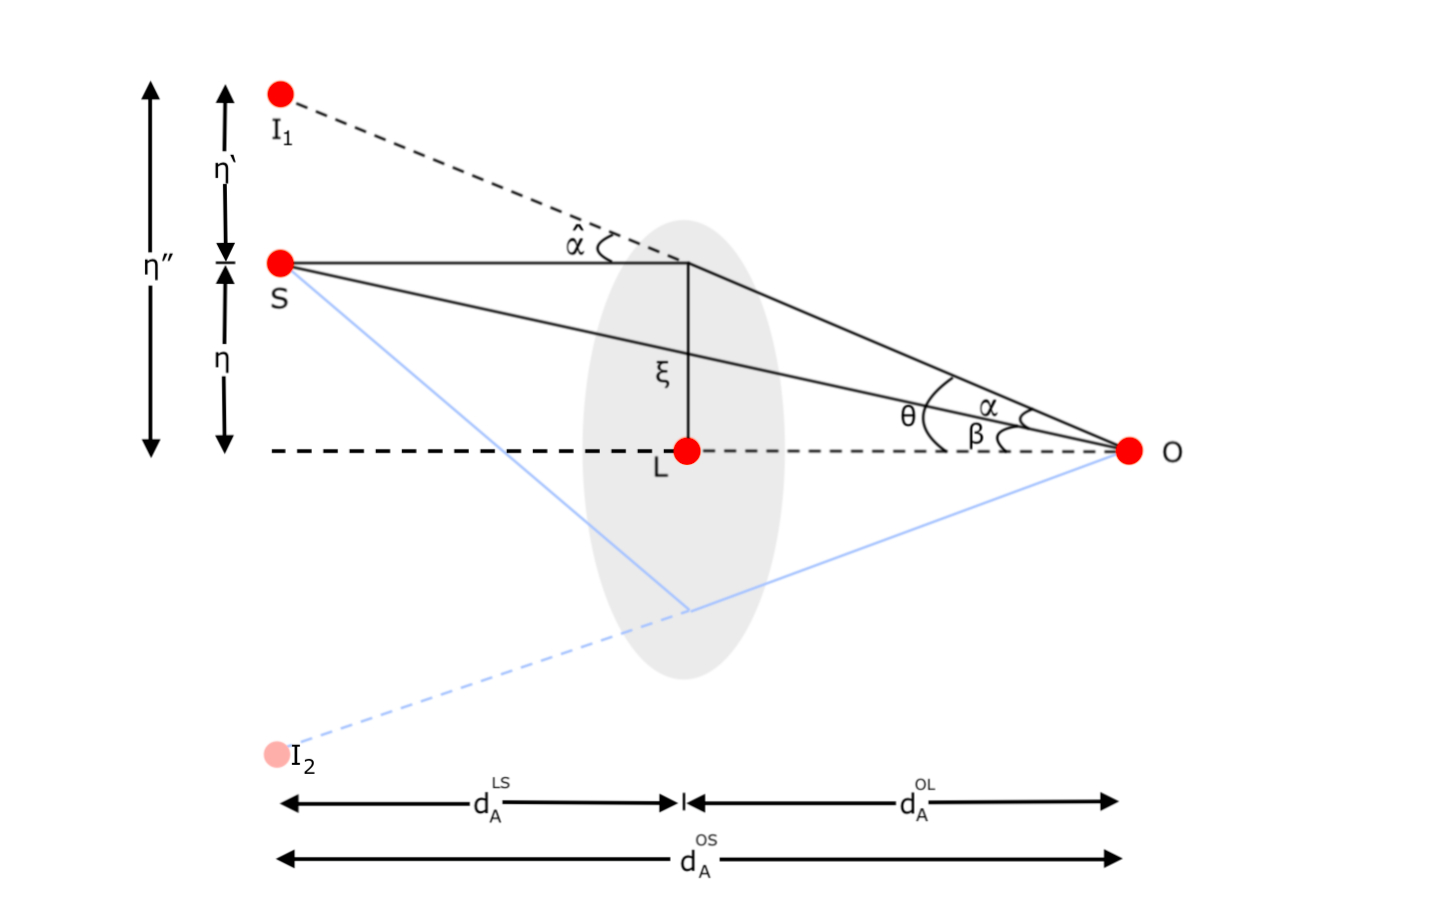
\includegraphics[width=90 mm]{sgl1}
%\caption{An observer at the origin observes a standard meter scale, of known proper length $\ell$, at comoving coordinate distance $r$.\\
%\label{fig:angull}}
\end{figure} 
\begin{center}
\begin{tikzpicture}[node distance=2cm]
\node (start) [startstop] {$\Delta t_{i j}=\dfrac{\left(1+z_{l}\right)}{2 c} \dfrac{d_{A}^{^{o s}} d_{A}^{^{o l}}}{d_{A}^{^{l s}}}\left[\theta_{j}^{2}-\theta_{i}^{2}\right]$};
\end{tikzpicture}
\end{center}
\end{frame}
 \begin{frame}
 \frametitle{DSR Method in Time Delay Distance}
 \vspace{3mm}
  \ding{74} For a Non-Euclidean geometry, comoving distances do not follow an additive Relation:
  $$
  d_{c o}^{^{\mathrm{ls}}}= d_\mathrm{c o}^{^\mathrm{os}} \sqrt{1+\Omega_{k0} \left(\dfrac{H_0}{c}d_\mathrm{c o}^\mathrm{^{ol}}\right)^{2}}-d_\mathrm{c o}^{^\mathrm{ol} }\sqrt{1+\Omega_{k0}\left(\dfrac{H_0}{c} d_\mathrm{c o}^{^\mathrm{os}}\right)^{2}}
  $$
%  \hspace{1cm}For $\boldsymbol{\Omega_{k0}=0}$
%  $$
%  d_\mathrm{c o}^{^{ls}}=d_\mathrm{c o}^{^\mathrm{os}}-d_\mathrm{c o}^{^\mathrm{ol}}
%  $$
  \ding{74}  Cosmic Distance Duality Parameter: $\eta=\dfrac{d_\mathrm{A}(1+z)^{2}}{d_\mathrm{L}}$
  \vspace{3mm}\\
 \ding{74} DSR in term of Time Delay Distance:
 \vspace{1mm}\\
\begin{footnotesize}
$$
{\tiny{ \dfrac{d_\mathrm{A}^{^\mathrm{o s}} d_\mathrm{A}^{^\mathrm{o l}}}{d_\mathrm{A}^{^\mathrm{l s}}}=\dfrac{1}{\left(1+z_{l}\right)}\left[\dfrac{\left(1+z_{l}\right)}{\eta_{l} d_\mathrm{L}^{^\mathrm{o l}}} \sqrt{1+\Omega_{k0}\left(\dfrac{\eta_{l} H_{0} d_\mathrm{L}^{^\mathrm{o l}}}{c\left(1+z_{l}\right)}\right)^{2}}-\dfrac{\left(1+z_{s}\right)}{\eta_{s} d_\mathrm{L}^{^\mathrm{o s}}} \sqrt{1+\Omega_{k0}\left(\dfrac{\eta_{s} H_{0} d_\mathrm{L}^{^ \mathrm{os}}}{c\left(1+z_{s}\right)}\right)^{2}}\right]^{-1}\hspace{1cm}}}
 $$
\end{footnotesize}
\end{frame}
\begin{frame}
 \frametitle{Observational Dataset-III}
\ding{74} \textbf{For Time Delay Distance in SGL systems:}\\\hspace{1cm} $\bullet$ Double-Imaged Lensed Dataset (12 Datapoints)\\
\hspace{1cm} $\bullet$ Recent H0LiCOW Dataset (6 Datapoints).
%12 data points: \hspace*{3 cm}$z_l\in[0.260,0.890]$ and \hspace*{0 cm}$z_s\in[0.944, 2.719]$
 \vspace{2mm}\\
\ding{74} \textbf{Statistical tools:}
 \begin{figure}[ht!]
\centering
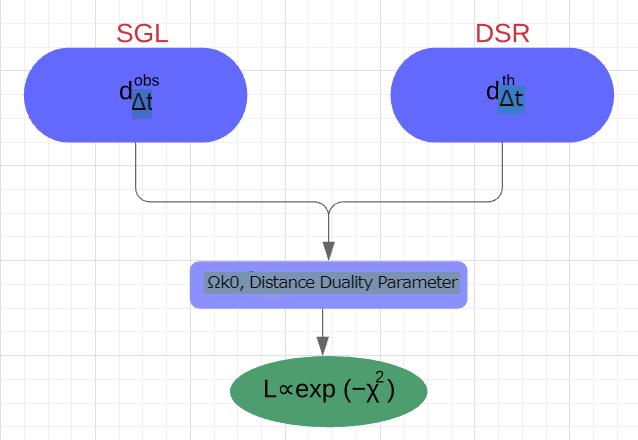
\includegraphics[width=80 mm]{flowchart_eicp1}
%\caption{An observer at the origin observes a standard meter scale, of known proper length $\ell$, at comoving coordinate distance $r$.\\
%\label{fig:angull}}
\end{figure} 
 \end{frame}
\begin{frame}
 \frametitle{Results: Time Delay Distance: P1}
\begin{small}
 
 $
{\boxed{\boldsymbol{\eta(z)=\eta_0}}}
$ 
\begin{table}
  \begin{tabular}{|c|c|c|}
    \hline
    \multirow{2}{*}{Dataset} &
      \multicolumn{2}{c|}{${\text { Best value }[68 \% \mathrm{CL}]}$} \\
\cline{2-3}
    &Double-Imaged Dataset & H0LiCOW Dataset \\
    \hline
    $\Omega_{k0}$ & $ {0.596_{-0.404}^{+0.287}}$ & $0.881^{+0.027}_{-0.020}$ \\
    \hline
    $ \eta_0$ &${0.828_{-0.045}^{+0.055}}$ &$1.641^{+0.253}_{-0.370}$  \\
       \hline
  \end{tabular}
\end{table}
\end{small}

 \begin{figure}[ht!]
\centering
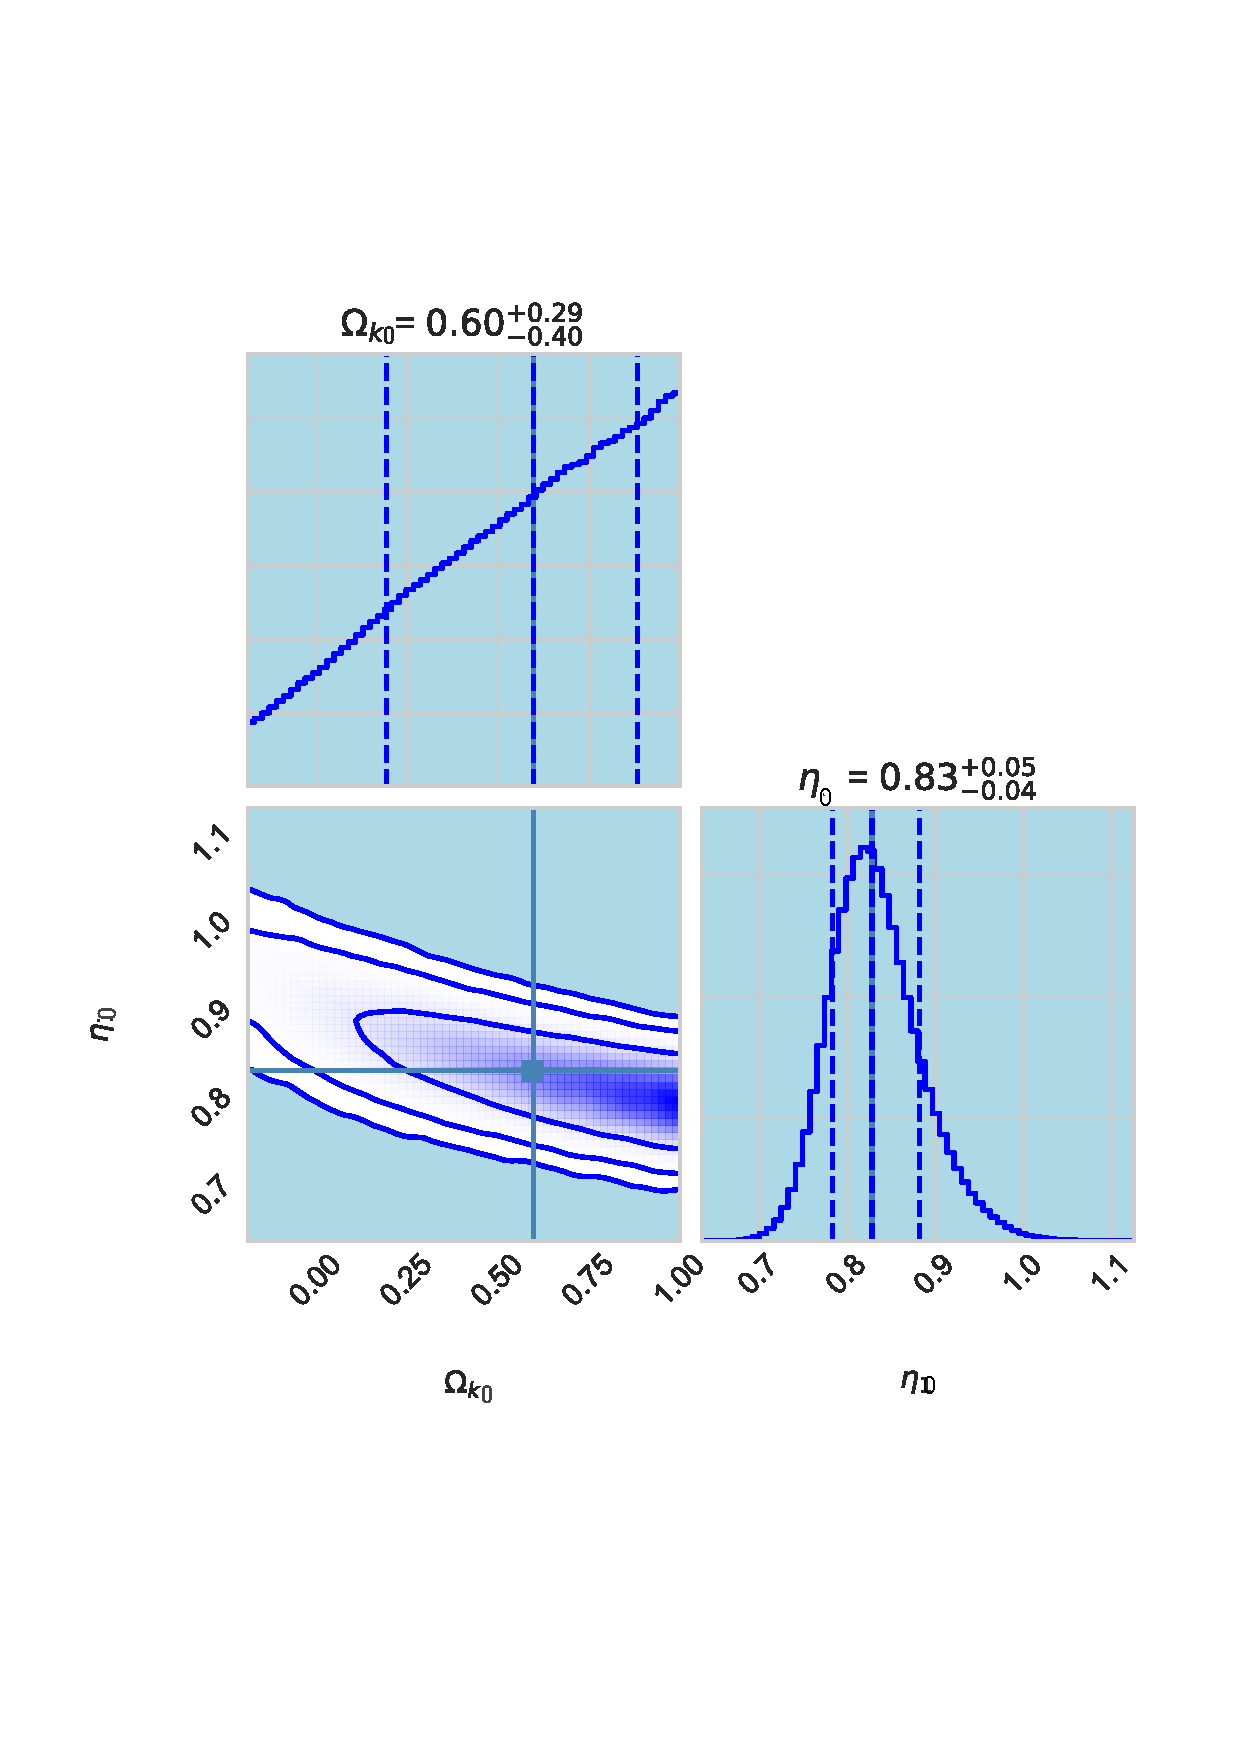
\includegraphics[width=45 mm]{rrrr}
\includegraphics[width=50 mm]{H0LiCOW_P1}
%\caption{An observer at the origin observes a standard meter scale, of known proper length $\ell$, at comoving coordinate distance $r$.\\
%\label{fig:angull}}
\end{figure} 
\end{frame}
\begin{frame}
 \frametitle{Results: Time Delay Distance: P2}
 $
{\boxed{\boldsymbol{\eta(z)=1+\eta_1z}}}
$
\begin{table}
  \begin{tabular}{|c|c|c|}
    \hline
    \multirow{2}{*}{Dataset} &
      \multicolumn{2}{c|}{${\text { Best value }[68 \% \mathrm{CL}]}$} \\
\cline{2-3}
    &Double-Imaged Dataset & H0LiCOW Dataset \\
    \hline
    $\Omega_{k0}$ & $ {0.050_{-0.037}^{+0.077}}$ &  $0.313^{+0.168}_{-0.196}$ \\
    \hline
    $ \eta_1$ &$ {0.118_{-0.110}^{+0.137}}$ & $0.249^{+0.173}_{-0.130}$  \\
       \hline
  \end{tabular}
\end{table}
%
% \hspace*{2cm}$\begin{array}
% {|c|c|c|}\hline 
% \text { Parameter } & {\text { Best value }[68 \% \mathrm{CL}]} \\ \hline 
% \Omega_{k} & {0.050_{-0.037}^{+0.077}} \\ \hline \eta_0 & {0.118_{-0.110}^{+0.137}} \\ \hline
% \end{array}$
 \begin{figure}[ht!]
\centering
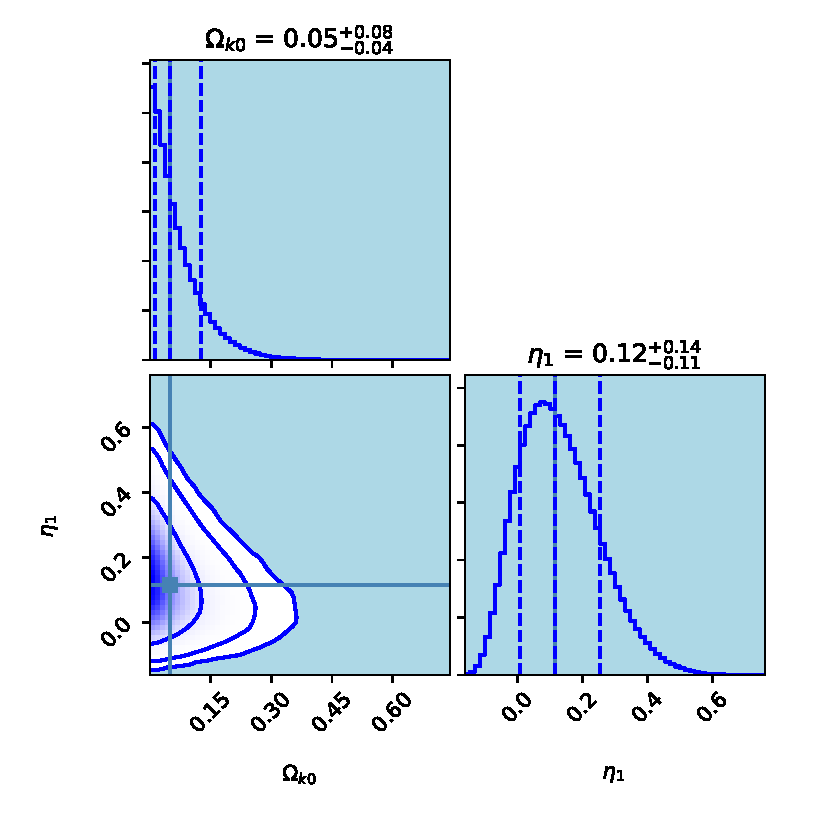
\includegraphics[width=45 mm]{time_delay_12_GRB_Pantheon_2nd_poly_P2_without_H0}
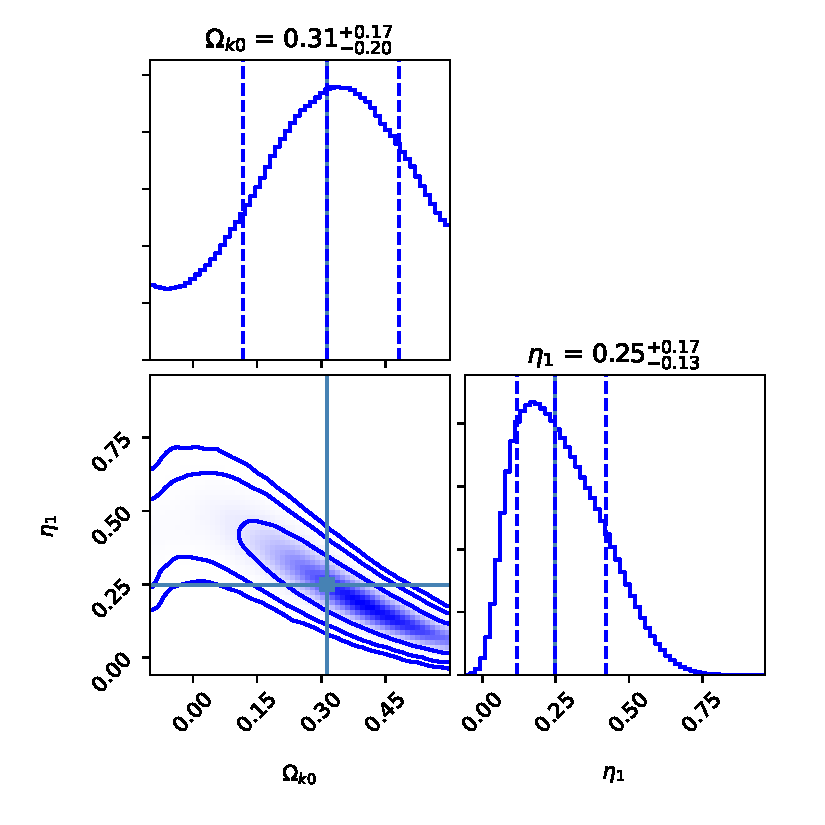
\includegraphics[width=45 mm]{H0LiCOW_P2}
%\caption{An observer at the origin observes a standard meter scale, of known proper length $\ell$, at comoving coordinate distance $r$.\\
%\label{fig:angull}}
\end{figure} 
\end{frame}
\begin{frame}
 \frametitle{Results: Time Delay Distance: P3}
 $
{\boxed{\boldsymbol{\eta(z)=1+\eta_1\dfrac{z}{1+z}}}}
$

\begin{table}
  \begin{tabular}{|c|c|c|}
    \hline
    \multirow{2}{*}{Dataset} &
      \multicolumn{2}{c|}{${\text { Best value }[68 \% \mathrm{CL}]}$} \\
\cline{2-3}
    &Double-Imaged Dataset & H0LiCOW Dataset \\
    \hline
    $\Omega_{k0}$ & $ {0.146_{-0.107}^{+0.209}}$ & $0.113^{+0.197}_{-0.144}$ \\
    \hline
    $ \eta_1$ &${-0.418_{-0.192}^{+0.227}}$ &  $0.344^{+0.195}_{-0.185}$  \\
       \hline
  \end{tabular}
\end{table}


% \hspace*{1.0cm}$\begin{array}
% {|c|c|c|}\hline 
% \text { Parameter } & {\text { Best value }[68 \% \mathrm{CL}]} \\ \hline 
% \Omega_{k} & {0.146_{-0.107}^{+0.209}} \\ \hline \eta_1 & {-0.418_{-0.192}^{+0.227}} \\ \hline
% \end{array}$
 \begin{figure}[ht!]
\centering
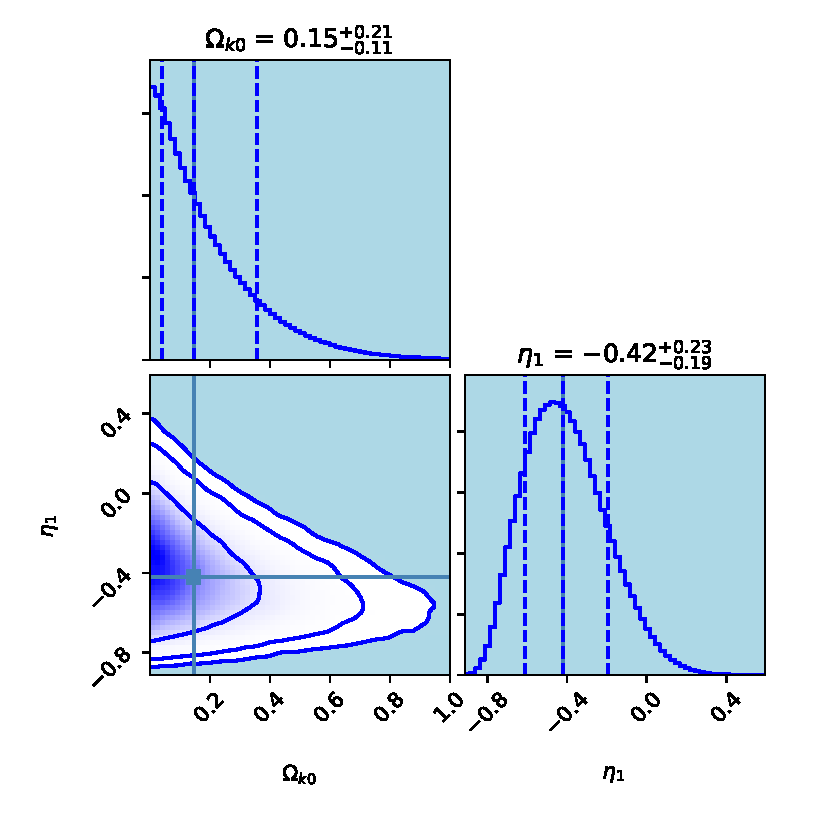
\includegraphics[width=43 mm]{time_delay_12_GRB_Pantheon_2nd_poly_P3_without_H0}
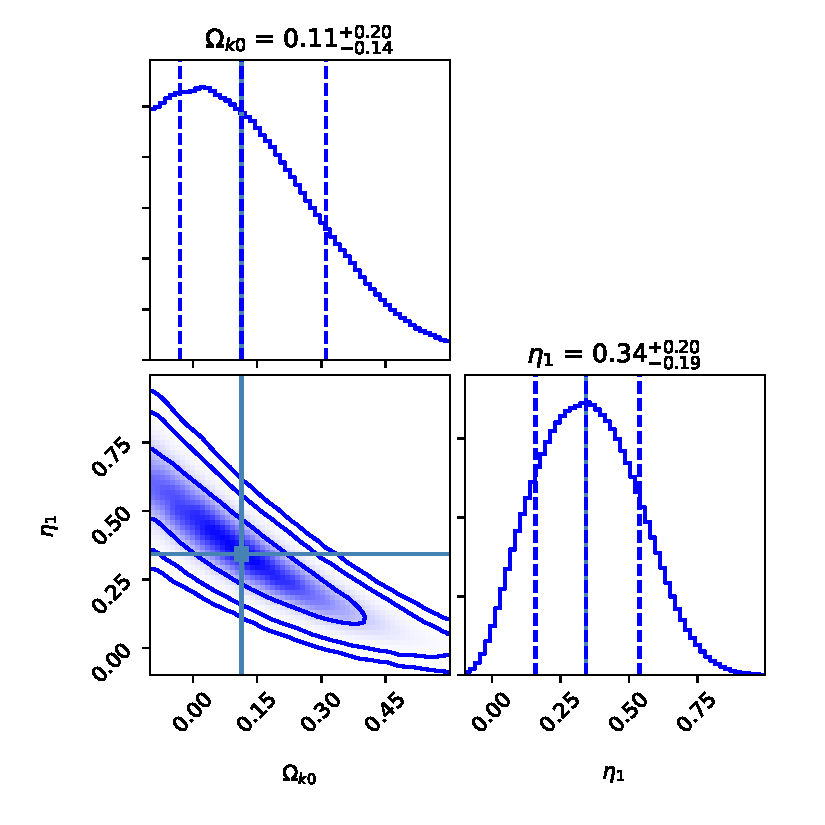
\includegraphics[width=43 mm]{H0LiCOW_P3}
%\caption{An observer at the origin observes a standard meter scale, of known proper length $\ell$, at comoving coordinate distance $r$.\\
%\label{fig:angull}}
\end{figure} 
\end{frame}
\begin{frame}
\frametitle{Conclusions: Time Delay Distance}
 \begin{itemize}
 \item
{ \textbf{\small {\color{red}$\eta(z)=\eta_0$}: Using double-imaged lensed dataset, the best fit value of $\Omega_{k0}$ suggests a spatially flat universe about  $95\%$ C.L. but H0LiCOW dataset shows an open universe even at $99\%$ C.L. Both dataset indicate a deviation in CDDR at $68\%$ C.L.
}}
\vspace{2mm}\\
 \item
\texttt{ \textbf{\small {\color{red}{$\eta(z)=1+\eta_1z$}}: The obtained value of  $\Omega_{k0}$ from both dataset supports a flat universe at $95\%$ C.L., while the value of distance duality parameter shows no violation $95\%$ C.L.}}
\vspace{2mm}\\
 \item
 \textbf{\small {\color{red}{$\eta(z)=1+\eta_1\dfrac{z}{1+z}$}}: Again the obtained value of $\Omega_{k0}$  is consistent with a flat universe from double-imaged lensed dataset and H0LiCOW dataset at $95\%$ and $68\%$ C.L. respectively. However the distance duality parameter shows a no violation from double-imaged lensed dataset and H0LiCOW dataset at $99\%$ and $95\%$ C.L. respectively.}


\end{itemize}
\end{frame}
\begin{frame}
 \frametitle{References}
 \begin{itemize}
 \item[1.]
 {\texttt {S. Serjeant, \emph{`` Observational cosmology''.} Cambridge University Press, 2010.}}
 \vspace{2mm}\\
 \item[2.]
{\texttt {S. R$\ddot{a}$s$\ddot{a}$nen et al, \emph{``New test of the Friedmann -Lema\^{i}tre-Robertson-Walker metric using the distance sum rule.''}  Phys. Rev. Lett. \textbf{115} (2015) 101301.}}
  \vspace{2mm}\\

 \item[3.]
{\texttt {J. Z. Qi et al, \emph{``The distance sum rule from strong lensing systems and quasars-test of cosmic curvature and beyond.''}  Mon. Not. Roy. Astron. Soc. \textbf{483} (2018) 1104}}
 \vspace{2mm}\\

\item[4.]
{\texttt {B. Wang et al, \emph{``Model-independent constraints on cosmic curvature from strong gravitational lensing and type Ia supernova observations.''} arXiv:1910.12173.}}
 \vspace{2mm}\\

\item[5.]
{\texttt {Y. Chen et al, \emph{``Assessing the effect of lens mass model in cosmological application with updated galaxy-scale strong gravitational lensing sample.''}  Mon. Not. Roy. Astron. Soc. \textbf{488} (2019) 3745.}}
\end{itemize}
 \end{frame}
{\1
\begin{frame}[plain,noframenumbering]
 
 {\color{blue}\Large \textbf{Workshop and Conferences:}}
 
\vspace{3mm}
  \begin{itemize}
 \item[\ding{74}]
Workshop on \textbf{``Applications of Data Science in Astrophysics and Gravitational Wave Research"}-November 1-4, 2019 IIIT Allahabad. I presented a \textbf{Poster Presentation.}
\vspace{3mm}\\
\item[\ding{74}]
International Conference on \textbf{``Gravitation \& Cosmology"}- December 10-13, 2019 IISER Mohali. In this International Conference, I presented a \textbf{Poster Presentation.}
\vspace{3mm}\\
\item[\ding{74}]
International Conference on \textbf{``Emerging Issues in Cosmology \& Particle Physics"}- January 12-14, 2020 Visva-Bharati, Shanti-Niketan. In this International Conference, I presented a \textbf{Oral talk Presentation.}
\vspace{8mm}\\
\item[]
\begin{center}
\textbf{Thank you for your attention !}
\end{center}
\end{itemize}
\end{frame}}
\end{document}
